\chapter{The Multi-Set Planning Problem}
\label{chap:multi-set}

This content is currently in submission \cite{dellin2015multiset}.

The purpose of this chapter is to introduce the multi-set planning
problem,
talk about its structure in general,
and show how about how a bunch of different problems in manipulation
are instances of this type of problem.

In the introduction to this chapter,
I'll talk about how the multi-step planning problem decomposition
discussed in Chapter~\ref{chap:formulation}
consists of a bunch of different queries in different
$\mathcal{C}_{\mbox{\scriptsize free}}$s, but that are related.

For example, say you're planning to move an object from an initial
location to a goal location,
and then move your manipulator back to the start pose.
See Figure~\ref{fig:manip-example}.
You have a single grasp for the object,
and your manipulator has a single IK for the grasp (very simple problem).
There are three $\mathcal{C}_{\mbox{\scriptsize free}}$s here;
a naive approach would plan separately in each.

\begin{figure}
\centering
\begin{subfigure}[b]{.45\linewidth}
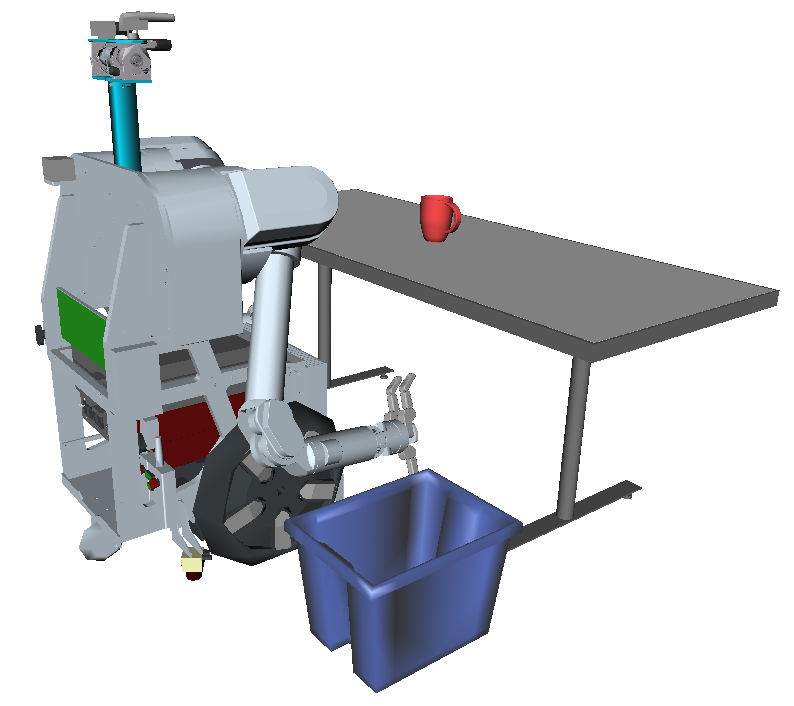
\includegraphics[width=\columnwidth]{figs/simple-table-clearing-task.png}
\end{subfigure}%
\quad%
\begin{subfigure}[b]{.45\linewidth}
\includegraphics{build/multiple-sets}
\end{subfigure}
\caption{
  The set of valid configurations for an articulated robot (left)
  changes often,
  especially in dynamic environments
  and multi-step manipulation problems.
  By describing this structure explicitly as set relations (right)
  and performing best-first search
  minimizing both planning and execution cost,
  we effectively reuse computation between similar
  problems.}
\label{fig:manip-example}
\end{figure}

\section{From RSS Intro}

Motion planning approaches that build graphs
in the collision-free subset of
\emph{configuration space} \cite{lozanoperez1983cspace},
e.g. the
PRM \cite{kavrakietal1996prm}
and RRT \cite{lavallekuffner1999rrt},
have proven promising
for high-dimensional articulated robotics problems
in unstructured environments.
These approaches devote a large amount of computational effort
testing configurations and paths for collision,
and the resulting graph can then be reused
for other queries in the same collision-free subset.

However,
for manipuation problems,
this subset of the robot's configuration space
is sensitive to the locations and shapes of
both people and objects in the environment,
as well as the robot itself.
In addition, it depends on the shape and pose of any object
grasped by the robot.
This makes it difficult not only to apply the results of prior
planning computation to the current problem,
but also to efficiently consider planned or hypothesized motions,
since we must reconstruct our graph from scratch whenever
the environment changes.
This is especially the case for
multi-step manipulation tasks that must be planned into the future.
%We want to continuously update our representation for detours.

A large body of prior work has focused on methods to
improve planning efficiency on manipulation problems,
which we review in Section~\ref{sec:related-work}.
Our first key insight is that many of these approaches are
in fact special instances of a more general structure,
which we formulate as the \emph{multi-set planning problem}
in Section~\ref{sec:multi-set}.

The Multi-Set PRM,
when applied to manipulation problems,
naturally produces an array of efficient behavior.
Section~\ref{sec:in-manipulation} outlines several such instances,
and also provides selected experimental results
on a multi-step manipulation task.
We also provide an open-source implementation of our algorithm.

\section{Motivation}

Imagine a simple ``pick and place'' manipulation planning scenario
in which an articulated robot in a novel cluttered environment
is tasked with moving a particular object from a start pose to a goal
pose in the scene.

\begin{figure}
\centering
\begin{subfigure}[b]{0.3\textwidth}
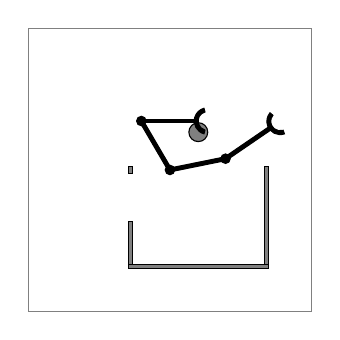
\begin{tikzpicture}
\begin{scope}[scale=1.2]
% bounding rect
\draw[color=black!50, thin] (-1.5,-1.5) rectangle (1.5,1.5);
\tikzstyle{dstyle}=[draw=black,fill=black!50]
\draw[dstyle] (0.300000,0.400000) circle (0.100000);
\draw[dstyle, shift={(0.300000,-1.020000)}, rotate=0.000000] (-0.740000,-0.020000) rectangle (0.740000,0.020000);
\draw[dstyle, shift={(1.020000,-0.480000)}, rotate=0.000000] (-0.020000,-0.520000) rectangle (0.020000,0.520000);
\draw[dstyle, shift={(-0.420000,-0.775000)}, rotate=0.000000] (-0.020000,-0.225000) rectangle (0.020000,0.225000);
\draw[dstyle, shift={(-0.420000,0.000000)}, rotate=0.000000] (-0.020000,-0.040000) rectangle (0.020000,0.040000);

\tikzstyle{dstyle}=[draw=black,fill=black]
\draw[dstyle] (0.000000,0.000000) circle (0.050000);
\draw[dstyle, shift={(0.294020,0.059601)}, rotate=11.459156] (-0.300000,-0.020000) rectangle (0.300000,0.020000);
\draw[dstyle] (0.588040,0.119202) circle (0.050000);
\draw[dstyle, shift={(1.165775,0.514451)}, rotate=214.377468](-74.484513:0.100000) arc (-74.484513:74.484513:0.100000) --(74.484513:0.140000) arc (74.484513:-74.484513:0.140000) -- cycle;
\draw[dstyle, shift={(0.835641,0.288594)}, rotate=34.377468] (-0.300000,-0.020000) rectangle (0.300000,0.020000);

%\tikzstyle{dstyle}=[draw=black!50]
%\draw[dstyle] (0.000000,0.000000) circle (0.050000);
\draw[dstyle, shift={(-0.151454,0.258963)}, rotate=120.321137] (-0.300000,-0.020000) rectangle (0.300000,0.020000);
\draw[dstyle] (-0.302908,0.517926) circle (0.050000);
\draw[dstyle, shift={(0.397092,0.517926)}, rotate=180.000000](-74.484513:0.100000) arc (-74.484513:74.484513:0.100000) --(74.484513:0.140000) arc (74.484513:-74.484513:0.140000) -- cycle;
\draw[dstyle, shift={(-0.002908,0.517926)}, rotate=0.000000] (-0.300000,-0.020000) rectangle (0.300000,0.020000);

\end{scope}
\end{tikzpicture}
\caption{Valid configuration}
\end{subfigure}%
\quad%
\begin{subfigure}[b]{0.3\textwidth}
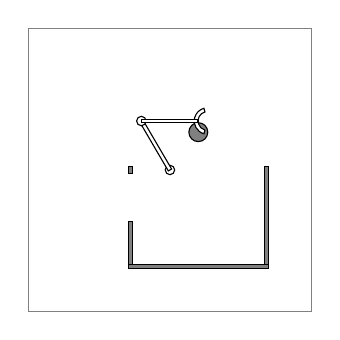
\begin{tikzpicture}
\begin{scope}[scale=1.2]
% bounding rect
\draw[color=black!50, thin] (-1.5,-1.5) rectangle (1.5,1.5);
\tikzstyle{dstyle}=[draw=black,fill=black!50]
\draw[dstyle] (0.300000,0.400000) circle (0.100000);
\draw[dstyle, shift={(0.300000,-1.020000)}, rotate=0.000000] (-0.740000,-0.020000) rectangle (0.740000,0.020000);
\draw[dstyle, shift={(1.020000,-0.480000)}, rotate=0.000000] (-0.020000,-0.520000) rectangle (0.020000,0.520000);
\draw[dstyle, shift={(-0.420000,-0.775000)}, rotate=0.000000] (-0.020000,-0.225000) rectangle (0.020000,0.225000);
\draw[dstyle, shift={(-0.420000,0.000000)}, rotate=0.000000] (-0.020000,-0.040000) rectangle (0.020000,0.040000);

\tikzstyle{dstyle}=[draw=black,fill=white]
\draw[dstyle] (0.000000,0.000000) circle (0.050000);
\draw[dstyle, shift={(-0.151454,0.258963)}, rotate=120.321137] (-0.300000,-0.020000) rectangle (0.300000,0.020000);
\draw[dstyle] (-0.302908,0.517926) circle (0.050000);
\draw[dstyle, shift={(0.397092,0.517926)}, rotate=180.000000](-74.484513:0.100000) arc (-74.484513:74.484513:0.100000) --(74.484513:0.140000) arc (74.484513:-74.484513:0.140000) -- cycle;
\draw[dstyle, shift={(-0.002908,0.517926)}, rotate=0.000000] (-0.300000,-0.020000) rectangle (0.300000,0.020000);

\end{scope}
\end{tikzpicture}
\caption{Invalid configuration}
\end{subfigure}%
\quad%
\begin{subfigure}[b]{0.3\textwidth}
\begin{tikzpicture}
\begin{scope}[scale=0.35]

\tikzstyle{every node}=[font=\scriptsize]

% x,y axes
\draw[->] (-3.14,-3.14) -- (4,-3.14) node[anchor=west] {$\theta_1$};
\draw[->] (-3.14,-3.14) -- (-3.14,4) node[anchor=south] {$\theta_2$};

% x tick marks with labels
\draw[-] (-3.14,-3.4) -- (-3.14,-3.14);
\draw[-] (    0,-3.4) -- (    0,-3.14);
\draw[-] ( 3.14,-3.4) -- ( 3.14,-3.14);
\draw	(-3.14,-3.4) node[anchor=north] {$-\pi$};
\draw	(    0,-3.4) node[anchor=north] {$0$};
\draw	( 3.14,-3.4) node[anchor=north] {$\pi$};

% y tick marks with labels
\draw[-] (-3.4,-3.14) -- (-3.14,-3.14);
\draw[-] (-3.4,    0) -- (-3.14,    0);
\draw[-] (-3.4, 3.14) -- (-3.14, 3.14);
\draw	(-3.4,-3.14) node[anchor=east] {$-\pi$};
\draw	(-3.4,    0) node[anchor=east] {$0$};
\draw	(-3.4, 3.14) node[anchor=east] {$\pi$};

% points
\draw[-,style=dotted] (0.2,-3.14) -- (0.2,0.4) -- (-3.14,0.4);
\draw[fill=black] (0.2,0.4) circle (0.15);
\draw[-,style=dotted] (2.1,-3.14) -- (2.1,-2.1) -- (-3.14,-2.1);
\draw[draw=black,fill=white] (2.1,-2.1) circle (0.15);

% legend
\draw[fill=black] (1,3.2) circle (0.15);
\draw	(1,3.2) node[anchor=west] {valid};
\draw[draw=black,fill=white] (1,2.3) circle (0.15);
\draw	(1,2.3) node[anchor=west] {invalid};

\end{scope}
\end{tikzpicture}
\caption{Configuration space}
\end{subfigure}
\caption{A simple planar 2-link manipulator problem.}
\end{figure}


\begin{figure}
\centering
\begin{subfigure}[b]{0.3\textwidth}
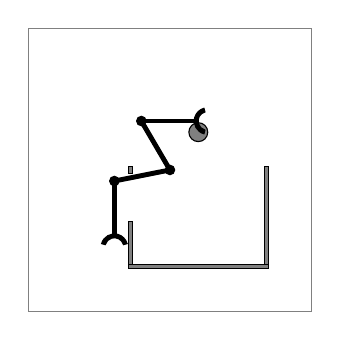
\begin{tikzpicture}
\begin{scope}[scale=1.2]
% bounding rect
\draw[color=black!50, thin] (-1.5,-1.5) rectangle (1.5,1.5);
\tikzstyle{dstyle}=[draw=black,fill=black!50]
\draw[dstyle] (0.300000,0.400000) circle (0.100000);
\draw[dstyle, shift={(0.300000,-1.020000)}, rotate=0.000000] (-0.740000,-0.020000) rectangle (0.740000,0.020000);
\draw[dstyle, shift={(1.020000,-0.480000)}, rotate=0.000000] (-0.020000,-0.520000) rectangle (0.020000,0.520000);
\draw[dstyle, shift={(-0.420000,-0.775000)}, rotate=0.000000] (-0.020000,-0.225000) rectangle (0.020000,0.225000);
\draw[dstyle, shift={(-0.420000,0.000000)}, rotate=0.000000] (-0.020000,-0.040000) rectangle (0.020000,0.040000);

\tikzstyle{dstyle}=[draw=black,fill=black]
\draw[dstyle] (0.000000,0.000000) circle (0.050000);
\draw[dstyle, shift={(-0.294233,-0.058540)}, rotate=-168.747530] (-0.300000,-0.020000) rectangle (0.300000,0.020000);
\draw[dstyle] (-0.588466,-0.117080) circle (0.050000);
\draw[dstyle, shift={(-0.588469,-0.817080)}, rotate=89.999790](-74.484513:0.100000) arc (-74.484513:74.484513:0.100000) --(74.484513:0.140000) arc (74.484513:-74.484513:0.140000) -- cycle;
\draw[dstyle, shift={(-0.588467,-0.417080)}, rotate=-90.000210] (-0.300000,-0.020000) rectangle (0.300000,0.020000);

%\tikzstyle{dstyle}=[draw=black!50]
%\draw[dstyle] (0.000000,0.000000) circle (0.050000);
\draw[dstyle, shift={(-0.151454,0.258963)}, rotate=120.321137] (-0.300000,-0.020000) rectangle (0.300000,0.020000);
\draw[dstyle] (-0.302908,0.517926) circle (0.050000);
\draw[dstyle, shift={(0.397092,0.517926)}, rotate=180.000000](-74.484513:0.100000) arc (-74.484513:74.484513:0.100000) --(74.484513:0.140000) arc (74.484513:-74.484513:0.140000) -- cycle;
\draw[dstyle, shift={(-0.002908,0.517926)}, rotate=0.000000] (-0.300000,-0.020000) rectangle (0.300000,0.020000);

\end{scope}
\end{tikzpicture}
\caption{Valid configuration}
\end{subfigure}%
\quad%
\begin{subfigure}[b]{0.3\textwidth}
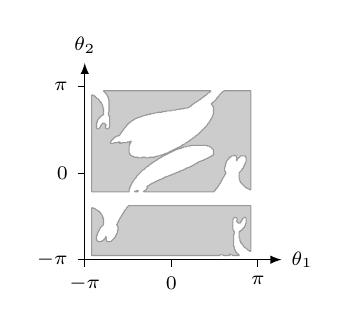
\begin{tikzpicture}
\begin{scope}[scale=0.35]

\tikzstyle{every node}=[font=\scriptsize]

% x,y axes
\draw[->] (-3.14,-3.14) -- (4,-3.14) node[anchor=west] {$\theta_1$};
\draw[->] (-3.14,-3.14) -- (-3.14,4) node[anchor=south] {$\theta_2$};

% x tick marks with labels
\draw[-] (-3.14,-3.4) -- (-3.14,-3.14);
\draw[-] (    0,-3.4) -- (    0,-3.14);
\draw[-] ( 3.14,-3.4) -- ( 3.14,-3.14);
\draw	(-3.14,-3.4) node[anchor=north] {$-\pi$};
\draw	(    0,-3.4) node[anchor=north] {$0$};
\draw	( 3.14,-3.4) node[anchor=north] {$\pi$};

% y tick marks with labels
\draw[-] (-3.4,-3.14) -- (-3.14,-3.14);
\draw[-] (-3.4,    0) -- (-3.14,    0);
\draw[-] (-3.4, 3.14) -- (-3.14, 3.14);
\draw	(-3.4,-3.14) node[anchor=east] {$-\pi$};
\draw	(-3.4,    0) node[anchor=east] {$0$};
\draw	(-3.4, 3.14) node[anchor=east] {$\pi$};

\begin{scope}[shift={(-3.14,-3.14)},scale=6.28]
\tikzstyle{fdstyle}=[color=black!40, fill=black!20, thin]
\filldraw[fdstyle, even odd rule]
   (0.254000,0.312000) -- (0.258000,0.312000) -- (0.262000,0.312000) -- (0.266000,0.312000) -- (0.270000,0.312000) -- (0.274000,0.312000) -- (0.278000,0.312000) -- (0.282000,0.312000) -- (0.286000,0.312000) -- (0.290000,0.312000) -- (0.294000,0.312000) -- (0.298000,0.312000) -- (0.302000,0.312000) -- (0.306000,0.312000) -- (0.310000,0.312000) -- (0.314000,0.312000) -- (0.318000,0.312000) -- (0.322000,0.312000) -- (0.326000,0.312000) -- (0.330000,0.312000) -- (0.334000,0.312000) -- (0.338000,0.312000) -- (0.342000,0.312000) -- (0.346000,0.312000) -- (0.350000,0.312000) -- (0.354000,0.312000) -- (0.358000,0.312000) -- (0.362000,0.312000) -- (0.366000,0.312000) -- (0.370000,0.312000) -- (0.374000,0.312000) -- (0.378000,0.312000) -- (0.382000,0.312000) -- (0.386000,0.312000) -- (0.390000,0.312000) -- (0.394000,0.312000) -- (0.398000,0.312000) -- (0.402000,0.312000) -- (0.406000,0.312000) -- (0.410000,0.312000) -- (0.414000,0.312000) -- (0.418000,0.312000) -- (0.422000,0.312000) -- (0.426000,0.312000) -- (0.430000,0.312000) -- (0.434000,0.312000) -- (0.438000,0.312000) -- (0.442000,0.312000) -- (0.446000,0.312000) -- (0.450000,0.312000) -- (0.454000,0.312000) -- (0.458000,0.312000) -- (0.462000,0.312000) -- (0.466000,0.312000) -- (0.470000,0.312000) -- (0.474000,0.312000) -- (0.478000,0.312000) -- (0.482000,0.312000) -- (0.486000,0.312000) -- (0.490000,0.312000) -- (0.494000,0.312000) -- (0.498000,0.312000) -- (0.502000,0.312000) -- (0.506000,0.312000) -- (0.510000,0.312000) -- (0.514000,0.312000) -- (0.518000,0.312000) -- (0.522000,0.312000) -- (0.526000,0.312000) -- (0.530000,0.312000) -- (0.534000,0.312000) -- (0.538000,0.312000) -- (0.542000,0.312000) -- (0.546000,0.312000) -- (0.550000,0.312000) -- (0.554000,0.312000) -- (0.558000,0.312000) -- (0.562000,0.312000) -- (0.566000,0.312000) -- (0.570000,0.312000) -- (0.574000,0.312000) -- (0.578000,0.312000) -- (0.582000,0.312000) -- (0.586000,0.312000) -- (0.590000,0.312000) -- (0.594000,0.312000) -- (0.598000,0.312000) -- (0.602000,0.312000) -- (0.606000,0.312000) -- (0.610000,0.312000) -- (0.614000,0.312000) -- (0.618000,0.312000) -- (0.622000,0.312000) -- (0.626000,0.312000) -- (0.630000,0.312000) -- (0.634000,0.312000) -- (0.638000,0.312000) -- (0.642000,0.312000) -- (0.646000,0.312000) -- (0.650000,0.312000) -- (0.654000,0.312000) -- (0.658000,0.312000) -- (0.662000,0.312000) -- (0.666000,0.312000) -- (0.670000,0.312000) -- (0.674000,0.312000) -- (0.678000,0.312000) -- (0.682000,0.312000) -- (0.686000,0.312000) -- (0.690000,0.312000) -- (0.694000,0.312000) -- (0.698000,0.312000) -- (0.702000,0.312000) -- (0.706000,0.312000) -- (0.710000,0.312000) -- (0.714000,0.312000) -- (0.718000,0.312000) -- (0.722000,0.312000) -- (0.726000,0.312000) -- (0.730000,0.312000) -- (0.734000,0.312000) -- (0.738000,0.312000) -- (0.742000,0.312000) -- (0.746000,0.312000) -- (0.750000,0.312000) -- (0.754000,0.312000) -- (0.758000,0.312000) -- (0.762000,0.312000) -- (0.766000,0.312000) -- (0.770000,0.312000) -- (0.774000,0.312000) -- (0.778000,0.312000) -- (0.782000,0.312000) -- (0.786000,0.312000) -- (0.790000,0.312000) -- (0.794000,0.312000) -- (0.798000,0.312000) -- (0.802000,0.312000) -- (0.806000,0.312000) -- (0.810000,0.312000) -- (0.814000,0.312000) -- (0.818000,0.312000) -- (0.822000,0.312000) -- (0.826000,0.312000) -- (0.830000,0.312000) -- (0.834000,0.312000) -- (0.838000,0.312000) -- (0.842000,0.312000) -- (0.846000,0.312000) -- (0.850000,0.312000) -- (0.854000,0.312000) -- (0.858000,0.312000) -- (0.862000,0.312000) -- (0.866000,0.312000) -- (0.870000,0.312000) -- (0.874000,0.312000) -- (0.878000,0.312000) -- (0.882000,0.312000) -- (0.886000,0.312000) -- (0.890000,0.312000) -- (0.894000,0.312000) -- (0.898000,0.312000) -- (0.902000,0.312000) -- (0.906000,0.312000) -- (0.910000,0.312000) -- (0.914000,0.312000) -- (0.918000,0.312000) -- (0.922000,0.312000) -- (0.926000,0.312000) -- (0.930000,0.312000) -- (0.934000,0.312000) -- (0.938000,0.312000) -- (0.942000,0.312000) -- (0.946000,0.312000) -- (0.950000,0.312000) -- (0.954000,0.312000) -- (0.958000,0.312000) -- (0.960000,0.310000) -- (0.960000,0.306000) -- (0.960000,0.302000) -- (0.960000,0.298000) -- (0.960000,0.294000) -- (0.960000,0.290000) -- (0.960000,0.286000) -- (0.960000,0.282000) -- (0.960000,0.278000) -- (0.960000,0.274000) -- (0.960000,0.270000) -- (0.960000,0.266000) -- (0.960000,0.262000) -- (0.960000,0.258000) -- (0.960000,0.254000) -- (0.960000,0.250000) -- (0.960000,0.246000) -- (0.960000,0.242000) -- (0.960000,0.238000) -- (0.960000,0.234000) -- (0.960000,0.230000) -- (0.960000,0.226000) -- (0.960000,0.222000) -- (0.960000,0.218000) -- (0.960000,0.214000) -- (0.960000,0.210000) -- (0.960000,0.206000) -- (0.960000,0.202000) -- (0.960000,0.198000) -- (0.960000,0.194000) -- (0.960000,0.190000) -- (0.960000,0.186000) -- (0.960000,0.182000) -- (0.960000,0.178000) -- (0.960000,0.174000) -- (0.960000,0.170000) -- (0.960000,0.166000) -- (0.960000,0.162000) -- (0.960000,0.158000) -- (0.960000,0.154000) -- (0.960000,0.150000) -- (0.960000,0.146000) -- (0.960000,0.142000) -- (0.960000,0.138000) -- (0.960000,0.134000) -- (0.960000,0.130000) -- (0.960000,0.126000) -- (0.960000,0.122000) -- (0.960000,0.118000) -- (0.960000,0.114000) -- (0.960000,0.110000) -- (0.960000,0.106000) -- (0.960000,0.102000) -- (0.960000,0.098000) -- (0.960000,0.094000) -- (0.960000,0.090000) -- (0.960000,0.086000) -- (0.960000,0.082000) -- (0.960000,0.078000) -- (0.960000,0.074000) -- (0.960000,0.070000) -- (0.960000,0.066000) -- (0.960000,0.062000) -- (0.960000,0.058000) -- (0.960000,0.054000) -- (0.960000,0.050000) -- (0.958000,0.048000) -- (0.954000,0.048000) -- (0.952000,0.050000) -- (0.950000,0.052000) -- (0.946000,0.052000) -- (0.944000,0.054000) -- (0.942000,0.056000) -- (0.940000,0.058000) -- (0.938000,0.060000) -- (0.936000,0.062000) -- (0.934000,0.064000) -- (0.932000,0.066000) -- (0.930000,0.068000) -- (0.926000,0.068000) -- (0.924000,0.070000) -- (0.922000,0.072000) -- (0.920000,0.074000) -- (0.918000,0.076000) -- (0.916000,0.078000) -- (0.916000,0.082000) -- (0.914000,0.084000) -- (0.912000,0.086000) -- (0.910000,0.088000) -- (0.908000,0.090000) -- (0.906000,0.092000) -- (0.904000,0.094000) -- (0.904000,0.098000) -- (0.902000,0.100000) -- (0.900000,0.102000) -- (0.900000,0.106000) -- (0.898000,0.108000) -- (0.896000,0.110000) -- (0.896000,0.114000) -- (0.896000,0.118000) -- (0.896000,0.122000) -- (0.894000,0.124000) -- (0.892000,0.126000) -- (0.892000,0.130000) -- (0.892000,0.134000) -- (0.892000,0.138000) -- (0.892000,0.142000) -- (0.892000,0.146000) -- (0.892000,0.150000) -- (0.892000,0.154000) -- (0.892000,0.158000) -- (0.892000,0.162000) -- (0.894000,0.164000) -- (0.898000,0.164000) -- (0.900000,0.166000) -- (0.902000,0.168000) -- (0.904000,0.170000) -- (0.906000,0.172000) -- (0.910000,0.172000) -- (0.912000,0.174000) -- (0.912000,0.178000) -- (0.914000,0.180000) -- (0.916000,0.182000) -- (0.918000,0.184000) -- (0.920000,0.186000) -- (0.922000,0.188000) -- (0.924000,0.190000) -- (0.924000,0.194000) -- (0.926000,0.196000) -- (0.928000,0.198000) -- (0.928000,0.202000) -- (0.928000,0.206000) -- (0.930000,0.208000) -- (0.932000,0.210000) -- (0.932000,0.214000) -- (0.932000,0.218000) -- (0.932000,0.222000) -- (0.932000,0.226000) -- (0.932000,0.230000) -- (0.932000,0.234000) -- (0.932000,0.238000) -- (0.932000,0.242000) -- (0.930000,0.244000) -- (0.926000,0.244000) -- (0.922000,0.244000) -- (0.920000,0.242000) -- (0.918000,0.240000) -- (0.914000,0.240000) -- (0.912000,0.238000) -- (0.912000,0.234000) -- (0.910000,0.232000) -- (0.908000,0.230000) -- (0.908000,0.226000) -- (0.906000,0.224000) -- (0.904000,0.222000) -- (0.902000,0.220000) -- (0.900000,0.218000) -- (0.900000,0.214000) -- (0.898000,0.212000) -- (0.894000,0.212000) -- (0.890000,0.212000) -- (0.886000,0.212000) -- (0.884000,0.214000) -- (0.882000,0.216000) -- (0.880000,0.218000) -- (0.878000,0.220000) -- (0.876000,0.222000) -- (0.878000,0.224000) -- (0.880000,0.226000) -- (0.880000,0.230000) -- (0.880000,0.234000) -- (0.880000,0.238000) -- (0.878000,0.240000) -- (0.876000,0.242000) -- (0.874000,0.244000) -- (0.870000,0.244000) -- (0.866000,0.244000) -- (0.864000,0.242000) -- (0.862000,0.240000) -- (0.860000,0.238000) -- (0.858000,0.236000) -- (0.856000,0.234000) -- (0.856000,0.230000) -- (0.856000,0.226000) -- (0.856000,0.222000) -- (0.856000,0.218000) -- (0.856000,0.214000) -- (0.856000,0.210000) -- (0.856000,0.206000) -- (0.856000,0.202000) -- (0.856000,0.198000) -- (0.856000,0.194000) -- (0.856000,0.190000) -- (0.856000,0.186000) -- (0.856000,0.182000) -- (0.856000,0.178000) -- (0.856000,0.174000) -- (0.858000,0.172000) -- (0.860000,0.170000) -- (0.860000,0.166000) -- (0.862000,0.164000) -- (0.864000,0.162000) -- (0.864000,0.158000) -- (0.864000,0.154000) -- (0.864000,0.150000) -- (0.862000,0.148000) -- (0.860000,0.146000) -- (0.860000,0.142000) -- (0.860000,0.138000) -- (0.860000,0.134000) -- (0.860000,0.130000) -- (0.860000,0.126000) -- (0.860000,0.122000) -- (0.860000,0.118000) -- (0.860000,0.114000) -- (0.860000,0.110000) -- (0.860000,0.106000) -- (0.860000,0.102000) -- (0.860000,0.098000) -- (0.860000,0.094000) -- (0.860000,0.090000) -- (0.860000,0.086000) -- (0.860000,0.082000) -- (0.860000,0.078000) -- (0.862000,0.076000) -- (0.864000,0.074000) -- (0.864000,0.070000) -- (0.864000,0.066000) -- (0.864000,0.062000) -- (0.866000,0.060000) -- (0.868000,0.058000) -- (0.868000,0.054000) -- (0.870000,0.052000) -- (0.872000,0.050000) -- (0.872000,0.046000) -- (0.874000,0.044000) -- (0.876000,0.042000) -- (0.878000,0.040000) -- (0.880000,0.038000) -- (0.882000,0.036000) -- (0.884000,0.034000) -- (0.886000,0.032000) -- (0.888000,0.030000) -- (0.890000,0.028000) -- (0.892000,0.026000) -- (0.890000,0.024000) -- (0.886000,0.024000) -- (0.882000,0.024000) -- (0.878000,0.024000) -- (0.874000,0.024000) -- (0.870000,0.024000) -- (0.866000,0.024000) -- (0.862000,0.024000) -- (0.858000,0.024000) -- (0.854000,0.024000) -- (0.852000,0.026000) -- (0.850000,0.028000) -- (0.846000,0.028000) -- (0.842000,0.028000) -- (0.840000,0.030000) -- (0.838000,0.032000) -- (0.836000,0.030000) -- (0.836000,0.026000) -- (0.834000,0.024000) -- (0.830000,0.024000) -- (0.826000,0.024000) -- (0.822000,0.024000) -- (0.818000,0.024000) -- (0.814000,0.024000) -- (0.810000,0.024000) -- (0.806000,0.024000) -- (0.802000,0.024000) -- (0.800000,0.026000) -- (0.798000,0.028000) -- (0.794000,0.028000) -- (0.790000,0.028000) -- (0.786000,0.028000) -- (0.782000,0.028000) -- (0.780000,0.026000) -- (0.778000,0.024000) -- (0.774000,0.024000) -- (0.770000,0.024000) -- (0.766000,0.024000) -- (0.762000,0.024000) -- (0.758000,0.024000) -- (0.754000,0.024000) -- (0.750000,0.024000) -- (0.746000,0.024000) -- (0.742000,0.024000) -- (0.738000,0.024000) -- (0.734000,0.024000) -- (0.730000,0.024000) -- (0.726000,0.024000) -- (0.722000,0.024000) -- (0.718000,0.024000) -- (0.714000,0.024000) -- (0.710000,0.024000) -- (0.706000,0.024000) -- (0.702000,0.024000) -- (0.698000,0.024000) -- (0.694000,0.024000) -- (0.690000,0.024000) -- (0.686000,0.024000) -- (0.682000,0.024000) -- (0.678000,0.024000) -- (0.674000,0.024000) -- (0.670000,0.024000) -- (0.666000,0.024000) -- (0.662000,0.024000) -- (0.658000,0.024000) -- (0.654000,0.024000) -- (0.650000,0.024000) -- (0.646000,0.024000) -- (0.642000,0.024000) -- (0.638000,0.024000) -- (0.634000,0.024000) -- (0.630000,0.024000) -- (0.626000,0.024000) -- (0.622000,0.024000) -- (0.618000,0.024000) -- (0.614000,0.024000) -- (0.610000,0.024000) -- (0.606000,0.024000) -- (0.602000,0.024000) -- (0.598000,0.024000) -- (0.594000,0.024000) -- (0.590000,0.024000) -- (0.586000,0.024000) -- (0.582000,0.024000) -- (0.578000,0.024000) -- (0.574000,0.024000) -- (0.570000,0.024000) -- (0.566000,0.024000) -- (0.562000,0.024000) -- (0.558000,0.024000) -- (0.554000,0.024000) -- (0.550000,0.024000) -- (0.546000,0.024000) -- (0.542000,0.024000) -- (0.538000,0.024000) -- (0.534000,0.024000) -- (0.530000,0.024000) -- (0.526000,0.024000) -- (0.522000,0.024000) -- (0.518000,0.024000) -- (0.514000,0.024000) -- (0.510000,0.024000) -- (0.506000,0.024000) -- (0.502000,0.024000) -- (0.498000,0.024000) -- (0.494000,0.024000) -- (0.490000,0.024000) -- (0.486000,0.024000) -- (0.482000,0.024000) -- (0.478000,0.024000) -- (0.474000,0.024000) -- (0.470000,0.024000) -- (0.466000,0.024000) -- (0.462000,0.024000) -- (0.458000,0.024000) -- (0.454000,0.024000) -- (0.450000,0.024000) -- (0.446000,0.024000) -- (0.442000,0.024000) -- (0.438000,0.024000) -- (0.434000,0.024000) -- (0.430000,0.024000) -- (0.426000,0.024000) -- (0.422000,0.024000) -- (0.418000,0.024000) -- (0.414000,0.024000) -- (0.410000,0.024000) -- (0.406000,0.024000) -- (0.402000,0.024000) -- (0.398000,0.024000) -- (0.394000,0.024000) -- (0.390000,0.024000) -- (0.386000,0.024000) -- (0.382000,0.024000) -- (0.378000,0.024000) -- (0.374000,0.024000) -- (0.370000,0.024000) -- (0.366000,0.024000) -- (0.362000,0.024000) -- (0.358000,0.024000) -- (0.354000,0.024000) -- (0.350000,0.024000) -- (0.346000,0.024000) -- (0.342000,0.024000) -- (0.338000,0.024000) -- (0.334000,0.024000) -- (0.330000,0.024000) -- (0.326000,0.024000) -- (0.322000,0.024000) -- (0.318000,0.024000) -- (0.314000,0.024000) -- (0.310000,0.024000) -- (0.306000,0.024000) -- (0.302000,0.024000) -- (0.298000,0.024000) -- (0.294000,0.024000) -- (0.290000,0.024000) -- (0.286000,0.024000) -- (0.282000,0.024000) -- (0.278000,0.024000) -- (0.274000,0.024000) -- (0.270000,0.024000) -- (0.266000,0.024000) -- (0.262000,0.024000) -- (0.258000,0.024000) -- (0.254000,0.024000) -- (0.250000,0.024000) -- (0.246000,0.024000) -- (0.242000,0.024000) -- (0.238000,0.024000) -- (0.234000,0.024000) -- (0.230000,0.024000) -- (0.226000,0.024000) -- (0.222000,0.024000) -- (0.218000,0.024000) -- (0.214000,0.024000) -- (0.210000,0.024000) -- (0.206000,0.024000) -- (0.202000,0.024000) -- (0.198000,0.024000) -- (0.194000,0.024000) -- (0.190000,0.024000) -- (0.186000,0.024000) -- (0.182000,0.024000) -- (0.178000,0.024000) -- (0.174000,0.024000) -- (0.170000,0.024000) -- (0.166000,0.024000) -- (0.162000,0.024000) -- (0.158000,0.024000) -- (0.154000,0.024000) -- (0.150000,0.024000) -- (0.146000,0.024000) -- (0.142000,0.024000) -- (0.138000,0.024000) -- (0.134000,0.024000) -- (0.130000,0.024000) -- (0.126000,0.024000) -- (0.122000,0.024000) -- (0.118000,0.024000) -- (0.114000,0.024000) -- (0.110000,0.024000) -- (0.106000,0.024000) -- (0.102000,0.024000) -- (0.098000,0.024000) -- (0.094000,0.024000) -- (0.090000,0.024000) -- (0.086000,0.024000) -- (0.082000,0.024000) -- (0.078000,0.024000) -- (0.074000,0.024000) -- (0.070000,0.024000) -- (0.066000,0.024000) -- (0.062000,0.024000) -- (0.058000,0.024000) -- (0.054000,0.024000) -- (0.050000,0.024000) -- (0.046000,0.024000) -- (0.042000,0.024000) -- (0.040000,0.026000) -- (0.040000,0.030000) -- (0.040000,0.034000) -- (0.040000,0.038000) -- (0.040000,0.042000) -- (0.040000,0.046000) -- (0.040000,0.050000) -- (0.040000,0.054000) -- (0.040000,0.058000) -- (0.040000,0.062000) -- (0.040000,0.066000) -- (0.040000,0.070000) -- (0.040000,0.074000) -- (0.040000,0.078000) -- (0.040000,0.082000) -- (0.040000,0.086000) -- (0.040000,0.090000) -- (0.040000,0.094000) -- (0.040000,0.098000) -- (0.040000,0.102000) -- (0.040000,0.106000) -- (0.040000,0.110000) -- (0.040000,0.114000) -- (0.040000,0.118000) -- (0.040000,0.122000) -- (0.040000,0.126000) -- (0.040000,0.130000) -- (0.040000,0.134000) -- (0.040000,0.138000) -- (0.040000,0.142000) -- (0.040000,0.146000) -- (0.040000,0.150000) -- (0.040000,0.154000) -- (0.040000,0.158000) -- (0.040000,0.162000) -- (0.040000,0.166000) -- (0.040000,0.170000) -- (0.040000,0.174000) -- (0.040000,0.178000) -- (0.040000,0.182000) -- (0.040000,0.186000) -- (0.040000,0.190000) -- (0.040000,0.194000) -- (0.040000,0.198000) -- (0.040000,0.202000) -- (0.040000,0.206000) -- (0.040000,0.210000) -- (0.040000,0.214000) -- (0.040000,0.218000) -- (0.040000,0.222000) -- (0.040000,0.226000) -- (0.040000,0.230000) -- (0.040000,0.234000) -- (0.040000,0.238000) -- (0.040000,0.242000) -- (0.040000,0.246000) -- (0.040000,0.250000) -- (0.040000,0.254000) -- (0.040000,0.258000) -- (0.040000,0.262000) -- (0.040000,0.266000) -- (0.040000,0.270000) -- (0.040000,0.274000) -- (0.040000,0.278000) -- (0.040000,0.282000) -- (0.040000,0.286000) -- (0.040000,0.290000) -- (0.040000,0.294000) -- (0.040000,0.298000) -- (0.042000,0.300000) -- (0.046000,0.300000) -- (0.048000,0.298000) -- (0.050000,0.296000) -- (0.054000,0.296000) -- (0.058000,0.296000) -- (0.060000,0.294000) -- (0.062000,0.292000) -- (0.064000,0.290000) -- (0.066000,0.288000) -- (0.070000,0.288000) -- (0.072000,0.286000) -- (0.074000,0.284000) -- (0.076000,0.282000) -- (0.078000,0.280000) -- (0.082000,0.280000) -- (0.084000,0.278000) -- (0.086000,0.276000) -- (0.088000,0.274000) -- (0.090000,0.272000) -- (0.092000,0.270000) -- (0.092000,0.266000) -- (0.094000,0.264000) -- (0.096000,0.262000) -- (0.098000,0.260000) -- (0.100000,0.258000) -- (0.100000,0.254000) -- (0.102000,0.252000) -- (0.104000,0.250000) -- (0.104000,0.246000) -- (0.104000,0.242000) -- (0.106000,0.240000) -- (0.108000,0.238000) -- (0.108000,0.234000) -- (0.108000,0.230000) -- (0.108000,0.226000) -- (0.108000,0.222000) -- (0.108000,0.218000) -- (0.108000,0.214000) -- (0.108000,0.210000) -- (0.108000,0.206000) -- (0.108000,0.202000) -- (0.106000,0.200000) -- (0.104000,0.198000) -- (0.102000,0.196000) -- (0.100000,0.194000) -- (0.098000,0.192000) -- (0.096000,0.190000) -- (0.094000,0.188000) -- (0.092000,0.186000) -- (0.090000,0.184000) -- (0.088000,0.182000) -- (0.088000,0.178000) -- (0.086000,0.176000) -- (0.084000,0.174000) -- (0.084000,0.170000) -- (0.082000,0.168000) -- (0.080000,0.166000) -- (0.080000,0.162000) -- (0.078000,0.160000) -- (0.076000,0.158000) -- (0.076000,0.154000) -- (0.074000,0.152000) -- (0.072000,0.150000) -- (0.072000,0.146000) -- (0.072000,0.142000) -- (0.070000,0.140000) -- (0.068000,0.138000) -- (0.068000,0.134000) -- (0.068000,0.130000) -- (0.068000,0.126000) -- (0.068000,0.122000) -- (0.068000,0.118000) -- (0.068000,0.114000) -- (0.070000,0.112000) -- (0.072000,0.110000) -- (0.074000,0.108000) -- (0.076000,0.106000) -- (0.078000,0.104000) -- (0.082000,0.104000) -- (0.086000,0.104000) -- (0.090000,0.104000) -- (0.094000,0.104000) -- (0.096000,0.106000) -- (0.098000,0.108000) -- (0.102000,0.108000) -- (0.104000,0.110000) -- (0.106000,0.112000) -- (0.108000,0.114000) -- (0.110000,0.116000) -- (0.112000,0.118000) -- (0.114000,0.120000) -- (0.116000,0.122000) -- (0.118000,0.124000) -- (0.120000,0.126000) -- (0.120000,0.130000) -- (0.122000,0.132000) -- (0.124000,0.130000) -- (0.124000,0.126000) -- (0.122000,0.124000) -- (0.120000,0.122000) -- (0.122000,0.120000) -- (0.124000,0.118000) -- (0.124000,0.114000) -- (0.124000,0.110000) -- (0.126000,0.108000) -- (0.128000,0.106000) -- (0.130000,0.104000) -- (0.134000,0.104000) -- (0.138000,0.104000) -- (0.142000,0.104000) -- (0.146000,0.104000) -- (0.150000,0.104000) -- (0.152000,0.106000) -- (0.154000,0.108000) -- (0.156000,0.110000) -- (0.158000,0.112000) -- (0.160000,0.114000) -- (0.162000,0.116000) -- (0.164000,0.118000) -- (0.166000,0.120000) -- (0.168000,0.122000) -- (0.170000,0.124000) -- (0.172000,0.126000) -- (0.174000,0.128000) -- (0.176000,0.130000) -- (0.176000,0.134000) -- (0.178000,0.136000) -- (0.180000,0.138000) -- (0.180000,0.142000) -- (0.182000,0.144000) -- (0.184000,0.146000) -- (0.184000,0.150000) -- (0.186000,0.152000) -- (0.188000,0.154000) -- (0.188000,0.158000) -- (0.188000,0.162000) -- (0.188000,0.166000) -- (0.190000,0.168000) -- (0.192000,0.170000) -- (0.192000,0.174000) -- (0.192000,0.178000) -- (0.192000,0.182000) -- (0.192000,0.186000) -- (0.192000,0.190000) -- (0.190000,0.192000) -- (0.188000,0.194000) -- (0.188000,0.198000) -- (0.186000,0.200000) -- (0.184000,0.202000) -- (0.186000,0.204000) -- (0.188000,0.206000) -- (0.188000,0.210000) -- (0.190000,0.212000) -- (0.192000,0.214000) -- (0.192000,0.218000) -- (0.194000,0.220000) -- (0.196000,0.222000) -- (0.196000,0.226000) -- (0.198000,0.228000) -- (0.200000,0.230000) -- (0.200000,0.234000) -- (0.202000,0.236000) -- (0.204000,0.238000) -- (0.204000,0.242000) -- (0.206000,0.244000) -- (0.208000,0.246000) -- (0.210000,0.248000) -- (0.212000,0.250000) -- (0.212000,0.254000) -- (0.214000,0.256000) -- (0.216000,0.258000) -- (0.216000,0.262000) -- (0.218000,0.264000) -- (0.220000,0.266000) -- (0.222000,0.268000) -- (0.224000,0.270000) -- (0.224000,0.274000) -- (0.226000,0.276000) -- (0.228000,0.278000) -- (0.228000,0.282000) -- (0.230000,0.284000) -- (0.232000,0.286000) -- (0.234000,0.288000) -- (0.236000,0.290000) -- (0.238000,0.292000) -- (0.240000,0.294000) -- (0.240000,0.298000) -- (0.242000,0.300000) -- (0.244000,0.302000) -- (0.246000,0.304000) -- (0.248000,0.306000) -- (0.250000,0.308000) -- (0.252000,0.310000) -- cycle
   (0.302000,0.400000) -- (0.306000,0.400000) -- (0.308000,0.398000) -- (0.308000,0.394000) -- (0.306000,0.392000) -- (0.302000,0.392000) -- (0.298000,0.392000) -- (0.294000,0.392000) -- (0.290000,0.392000) -- (0.288000,0.394000) -- (0.290000,0.396000) -- (0.294000,0.396000) -- (0.298000,0.396000) -- (0.300000,0.398000) -- cycle
   (0.110000,0.976000) -- (0.114000,0.976000) -- (0.118000,0.976000) -- (0.122000,0.976000) -- (0.126000,0.976000) -- (0.130000,0.976000) -- (0.134000,0.976000) -- (0.138000,0.976000) -- (0.142000,0.976000) -- (0.146000,0.976000) -- (0.150000,0.976000) -- (0.154000,0.976000) -- (0.158000,0.976000) -- (0.162000,0.976000) -- (0.166000,0.976000) -- (0.170000,0.976000) -- (0.174000,0.976000) -- (0.178000,0.976000) -- (0.182000,0.976000) -- (0.186000,0.976000) -- (0.190000,0.976000) -- (0.194000,0.976000) -- (0.198000,0.976000) -- (0.202000,0.976000) -- (0.206000,0.976000) -- (0.210000,0.976000) -- (0.214000,0.976000) -- (0.218000,0.976000) -- (0.222000,0.976000) -- (0.226000,0.976000) -- (0.230000,0.976000) -- (0.234000,0.976000) -- (0.238000,0.976000) -- (0.242000,0.976000) -- (0.246000,0.976000) -- (0.250000,0.976000) -- (0.254000,0.976000) -- (0.258000,0.976000) -- (0.262000,0.976000) -- (0.266000,0.976000) -- (0.270000,0.976000) -- (0.274000,0.976000) -- (0.278000,0.976000) -- (0.282000,0.976000) -- (0.286000,0.976000) -- (0.290000,0.976000) -- (0.294000,0.976000) -- (0.298000,0.976000) -- (0.302000,0.976000) -- (0.306000,0.976000) -- (0.310000,0.976000) -- (0.314000,0.976000) -- (0.318000,0.976000) -- (0.322000,0.976000) -- (0.326000,0.976000) -- (0.330000,0.976000) -- (0.334000,0.976000) -- (0.338000,0.976000) -- (0.342000,0.976000) -- (0.346000,0.976000) -- (0.350000,0.976000) -- (0.354000,0.976000) -- (0.358000,0.976000) -- (0.362000,0.976000) -- (0.366000,0.976000) -- (0.370000,0.976000) -- (0.374000,0.976000) -- (0.378000,0.976000) -- (0.382000,0.976000) -- (0.386000,0.976000) -- (0.390000,0.976000) -- (0.394000,0.976000) -- (0.398000,0.976000) -- (0.402000,0.976000) -- (0.406000,0.976000) -- (0.410000,0.976000) -- (0.414000,0.976000) -- (0.418000,0.976000) -- (0.422000,0.976000) -- (0.426000,0.976000) -- (0.430000,0.976000) -- (0.434000,0.976000) -- (0.438000,0.976000) -- (0.442000,0.976000) -- (0.446000,0.976000) -- (0.450000,0.976000) -- (0.454000,0.976000) -- (0.458000,0.976000) -- (0.462000,0.976000) -- (0.466000,0.976000) -- (0.470000,0.976000) -- (0.474000,0.976000) -- (0.478000,0.976000) -- (0.482000,0.976000) -- (0.486000,0.976000) -- (0.490000,0.976000) -- (0.494000,0.976000) -- (0.498000,0.976000) -- (0.502000,0.976000) -- (0.506000,0.976000) -- (0.510000,0.976000) -- (0.514000,0.976000) -- (0.518000,0.976000) -- (0.522000,0.976000) -- (0.526000,0.976000) -- (0.530000,0.976000) -- (0.534000,0.976000) -- (0.538000,0.976000) -- (0.542000,0.976000) -- (0.546000,0.976000) -- (0.550000,0.976000) -- (0.554000,0.976000) -- (0.558000,0.976000) -- (0.562000,0.976000) -- (0.566000,0.976000) -- (0.570000,0.976000) -- (0.574000,0.976000) -- (0.578000,0.976000) -- (0.582000,0.976000) -- (0.586000,0.976000) -- (0.590000,0.976000) -- (0.594000,0.976000) -- (0.598000,0.976000) -- (0.602000,0.976000) -- (0.606000,0.976000) -- (0.610000,0.976000) -- (0.614000,0.976000) -- (0.618000,0.976000) -- (0.622000,0.976000) -- (0.626000,0.976000) -- (0.630000,0.976000) -- (0.634000,0.976000) -- (0.638000,0.976000) -- (0.642000,0.976000) -- (0.646000,0.976000) -- (0.650000,0.976000) -- (0.654000,0.976000) -- (0.658000,0.976000) -- (0.662000,0.976000) -- (0.666000,0.976000) -- (0.670000,0.976000) -- (0.674000,0.976000) -- (0.678000,0.976000) -- (0.682000,0.976000) -- (0.686000,0.976000) -- (0.690000,0.976000) -- (0.694000,0.976000) -- (0.698000,0.976000) -- (0.702000,0.976000) -- (0.706000,0.976000) -- (0.710000,0.976000) -- (0.714000,0.976000) -- (0.718000,0.976000) -- (0.722000,0.976000) -- (0.726000,0.976000) -- (0.728000,0.974000) -- (0.726000,0.972000) -- (0.724000,0.970000) -- (0.722000,0.968000) -- (0.720000,0.966000) -- (0.718000,0.964000) -- (0.714000,0.964000) -- (0.712000,0.962000) -- (0.710000,0.960000) -- (0.708000,0.958000) -- (0.706000,0.956000) -- (0.704000,0.954000) -- (0.702000,0.952000) -- (0.700000,0.950000) -- (0.698000,0.948000) -- (0.694000,0.948000) -- (0.692000,0.946000) -- (0.690000,0.944000) -- (0.688000,0.942000) -- (0.686000,0.940000) -- (0.684000,0.938000) -- (0.682000,0.936000) -- (0.678000,0.936000) -- (0.676000,0.934000) -- (0.674000,0.932000) -- (0.672000,0.930000) -- (0.670000,0.928000) -- (0.668000,0.926000) -- (0.666000,0.924000) -- (0.662000,0.924000) -- (0.660000,0.922000) -- (0.658000,0.920000) -- (0.656000,0.918000) -- (0.654000,0.916000) -- (0.650000,0.916000) -- (0.648000,0.914000) -- (0.646000,0.912000) -- (0.644000,0.910000) -- (0.642000,0.908000) -- (0.638000,0.908000) -- (0.636000,0.906000) -- (0.634000,0.904000) -- (0.632000,0.902000) -- (0.630000,0.900000) -- (0.626000,0.900000) -- (0.624000,0.898000) -- (0.622000,0.896000) -- (0.620000,0.894000) -- (0.618000,0.892000) -- (0.616000,0.890000) -- (0.614000,0.888000) -- (0.610000,0.888000) -- (0.608000,0.886000) -- (0.606000,0.884000) -- (0.604000,0.882000) -- (0.602000,0.880000) -- (0.598000,0.880000) -- (0.596000,0.878000) -- (0.594000,0.876000) -- (0.590000,0.876000) -- (0.586000,0.876000) -- (0.582000,0.876000) -- (0.578000,0.876000) -- (0.576000,0.874000) -- (0.574000,0.872000) -- (0.570000,0.872000) -- (0.566000,0.872000) -- (0.562000,0.872000) -- (0.558000,0.872000) -- (0.554000,0.872000) -- (0.552000,0.870000) -- (0.550000,0.868000) -- (0.546000,0.868000) -- (0.542000,0.868000) -- (0.538000,0.868000) -- (0.534000,0.868000) -- (0.530000,0.868000) -- (0.528000,0.866000) -- (0.526000,0.864000) -- (0.522000,0.864000) -- (0.518000,0.864000) -- (0.514000,0.864000) -- (0.510000,0.864000) -- (0.506000,0.864000) -- (0.502000,0.864000) -- (0.500000,0.862000) -- (0.498000,0.860000) -- (0.494000,0.860000) -- (0.490000,0.860000) -- (0.486000,0.860000) -- (0.482000,0.860000) -- (0.478000,0.860000) -- (0.474000,0.860000) -- (0.472000,0.858000) -- (0.470000,0.856000) -- (0.466000,0.856000) -- (0.462000,0.856000) -- (0.458000,0.856000) -- (0.454000,0.856000) -- (0.450000,0.856000) -- (0.448000,0.854000) -- (0.446000,0.852000) -- (0.442000,0.852000) -- (0.438000,0.852000) -- (0.434000,0.852000) -- (0.430000,0.852000) -- (0.426000,0.852000) -- (0.422000,0.852000) -- (0.420000,0.850000) -- (0.418000,0.848000) -- (0.414000,0.848000) -- (0.410000,0.848000) -- (0.406000,0.848000) -- (0.402000,0.848000) -- (0.400000,0.846000) -- (0.398000,0.844000) -- (0.394000,0.844000) -- (0.390000,0.844000) -- (0.386000,0.844000) -- (0.382000,0.844000) -- (0.380000,0.842000) -- (0.378000,0.840000) -- (0.374000,0.840000) -- (0.370000,0.840000) -- (0.366000,0.840000) -- (0.364000,0.838000) -- (0.362000,0.836000) -- (0.358000,0.836000) -- (0.354000,0.836000) -- (0.350000,0.836000) -- (0.348000,0.834000) -- (0.346000,0.832000) -- (0.342000,0.832000) -- (0.338000,0.832000) -- (0.336000,0.830000) -- (0.334000,0.828000) -- (0.330000,0.828000) -- (0.326000,0.828000) -- (0.324000,0.826000) -- (0.322000,0.824000) -- (0.318000,0.824000) -- (0.314000,0.824000) -- (0.312000,0.822000) -- (0.310000,0.820000) -- (0.306000,0.820000) -- (0.302000,0.820000) -- (0.300000,0.818000) -- (0.298000,0.816000) -- (0.294000,0.816000) -- (0.292000,0.814000) -- (0.290000,0.812000) -- (0.286000,0.812000) -- (0.284000,0.810000) -- (0.282000,0.808000) -- (0.280000,0.806000) -- (0.278000,0.804000) -- (0.274000,0.804000) -- (0.272000,0.802000) -- (0.270000,0.800000) -- (0.268000,0.798000) -- (0.266000,0.796000) -- (0.264000,0.794000) -- (0.262000,0.792000) -- (0.258000,0.792000) -- (0.256000,0.790000) -- (0.254000,0.788000) -- (0.252000,0.786000) -- (0.250000,0.784000) -- (0.248000,0.782000) -- (0.246000,0.780000) -- (0.244000,0.778000) -- (0.242000,0.776000) -- (0.240000,0.774000) -- (0.240000,0.770000) -- (0.238000,0.768000) -- (0.236000,0.766000) -- (0.234000,0.764000) -- (0.232000,0.762000) -- (0.230000,0.760000) -- (0.228000,0.758000) -- (0.226000,0.756000) -- (0.224000,0.754000) -- (0.224000,0.750000) -- (0.222000,0.748000) -- (0.220000,0.746000) -- (0.218000,0.744000) -- (0.216000,0.742000) -- (0.214000,0.740000) -- (0.212000,0.738000) -- (0.212000,0.734000) -- (0.210000,0.732000) -- (0.208000,0.730000) -- (0.206000,0.728000) -- (0.204000,0.726000) -- (0.204000,0.722000) -- (0.202000,0.720000) -- (0.200000,0.718000) -- (0.198000,0.716000) -- (0.194000,0.716000) -- (0.190000,0.716000) -- (0.188000,0.714000) -- (0.186000,0.712000) -- (0.182000,0.712000) -- (0.180000,0.710000) -- (0.178000,0.708000) -- (0.174000,0.708000) -- (0.172000,0.706000) -- (0.170000,0.704000) -- (0.168000,0.702000) -- (0.166000,0.700000) -- (0.164000,0.698000) -- (0.162000,0.696000) -- (0.160000,0.694000) -- (0.158000,0.692000) -- (0.156000,0.690000) -- (0.154000,0.688000) -- (0.152000,0.686000) -- (0.152000,0.682000) -- (0.150000,0.680000) -- (0.148000,0.678000) -- (0.148000,0.674000) -- (0.150000,0.672000) -- (0.154000,0.672000) -- (0.158000,0.672000) -- (0.162000,0.672000) -- (0.166000,0.672000) -- (0.168000,0.674000) -- (0.170000,0.676000) -- (0.174000,0.676000) -- (0.178000,0.676000) -- (0.182000,0.676000) -- (0.186000,0.676000) -- (0.190000,0.676000) -- (0.192000,0.678000) -- (0.194000,0.680000) -- (0.198000,0.680000) -- (0.202000,0.680000) -- (0.204000,0.678000) -- (0.202000,0.676000) -- (0.200000,0.674000) -- (0.202000,0.672000) -- (0.206000,0.672000) -- (0.210000,0.672000) -- (0.214000,0.672000) -- (0.216000,0.674000) -- (0.218000,0.676000) -- (0.222000,0.676000) -- (0.226000,0.676000) -- (0.230000,0.676000) -- (0.234000,0.676000) -- (0.238000,0.676000) -- (0.242000,0.676000) -- (0.244000,0.678000) -- (0.246000,0.680000) -- (0.250000,0.680000) -- (0.254000,0.680000) -- (0.258000,0.680000) -- (0.260000,0.682000) -- (0.262000,0.684000) -- (0.266000,0.684000) -- (0.268000,0.682000) -- (0.266000,0.680000) -- (0.264000,0.678000) -- (0.264000,0.674000) -- (0.262000,0.672000) -- (0.260000,0.670000) -- (0.260000,0.666000) -- (0.260000,0.662000) -- (0.258000,0.660000) -- (0.256000,0.658000) -- (0.256000,0.654000) -- (0.256000,0.650000) -- (0.256000,0.646000) -- (0.256000,0.642000) -- (0.256000,0.638000) -- (0.256000,0.634000) -- (0.256000,0.630000) -- (0.256000,0.626000) -- (0.256000,0.622000) -- (0.256000,0.618000) -- (0.258000,0.616000) -- (0.260000,0.614000) -- (0.260000,0.610000) -- (0.262000,0.608000) -- (0.264000,0.606000) -- (0.266000,0.604000) -- (0.268000,0.602000) -- (0.270000,0.600000) -- (0.274000,0.600000) -- (0.276000,0.598000) -- (0.278000,0.596000) -- (0.282000,0.596000) -- (0.284000,0.594000) -- (0.286000,0.592000) -- (0.290000,0.592000) -- (0.294000,0.592000) -- (0.298000,0.592000) -- (0.302000,0.592000) -- (0.306000,0.592000) -- (0.308000,0.590000) -- (0.310000,0.588000) -- (0.314000,0.588000) -- (0.318000,0.588000) -- (0.322000,0.588000) -- (0.326000,0.588000) -- (0.328000,0.590000) -- (0.330000,0.592000) -- (0.334000,0.592000) -- (0.338000,0.592000) -- (0.342000,0.592000) -- (0.346000,0.592000) -- (0.350000,0.592000) -- (0.352000,0.590000) -- (0.354000,0.588000) -- (0.358000,0.588000) -- (0.362000,0.588000) -- (0.366000,0.588000) -- (0.370000,0.588000) -- (0.372000,0.590000) -- (0.374000,0.592000) -- (0.378000,0.592000) -- (0.382000,0.592000) -- (0.386000,0.592000) -- (0.390000,0.592000) -- (0.394000,0.592000) -- (0.398000,0.592000) -- (0.402000,0.592000) -- (0.404000,0.594000) -- (0.406000,0.596000) -- (0.410000,0.596000) -- (0.414000,0.596000) -- (0.418000,0.596000) -- (0.420000,0.598000) -- (0.422000,0.600000) -- (0.426000,0.600000) -- (0.430000,0.600000) -- (0.434000,0.600000) -- (0.436000,0.602000) -- (0.438000,0.604000) -- (0.442000,0.604000) -- (0.446000,0.604000) -- (0.448000,0.606000) -- (0.450000,0.608000) -- (0.454000,0.608000) -- (0.458000,0.608000) -- (0.460000,0.610000) -- (0.462000,0.612000) -- (0.466000,0.612000) -- (0.468000,0.614000) -- (0.470000,0.616000) -- (0.474000,0.616000) -- (0.478000,0.616000) -- (0.480000,0.618000) -- (0.482000,0.620000) -- (0.486000,0.620000) -- (0.488000,0.622000) -- (0.490000,0.624000) -- (0.494000,0.624000) -- (0.496000,0.626000) -- (0.498000,0.628000) -- (0.502000,0.628000) -- (0.504000,0.630000) -- (0.506000,0.632000) -- (0.510000,0.632000) -- (0.512000,0.634000) -- (0.514000,0.636000) -- (0.518000,0.636000) -- (0.520000,0.638000) -- (0.522000,0.640000) -- (0.526000,0.640000) -- (0.528000,0.642000) -- (0.530000,0.644000) -- (0.534000,0.644000) -- (0.536000,0.646000) -- (0.538000,0.648000) -- (0.542000,0.648000) -- (0.544000,0.650000) -- (0.546000,0.652000) -- (0.550000,0.652000) -- (0.552000,0.654000) -- (0.554000,0.656000) -- (0.558000,0.656000) -- (0.560000,0.658000) -- (0.562000,0.660000) -- (0.564000,0.662000) -- (0.566000,0.664000) -- (0.570000,0.664000) -- (0.572000,0.666000) -- (0.574000,0.668000) -- (0.578000,0.668000) -- (0.580000,0.670000) -- (0.582000,0.672000) -- (0.584000,0.674000) -- (0.586000,0.676000) -- (0.590000,0.676000) -- (0.592000,0.678000) -- (0.594000,0.680000) -- (0.596000,0.682000) -- (0.598000,0.684000) -- (0.602000,0.684000) -- (0.604000,0.686000) -- (0.606000,0.688000) -- (0.608000,0.690000) -- (0.610000,0.692000) -- (0.614000,0.692000) -- (0.616000,0.694000) -- (0.618000,0.696000) -- (0.620000,0.698000) -- (0.622000,0.700000) -- (0.624000,0.702000) -- (0.626000,0.704000) -- (0.630000,0.704000) -- (0.632000,0.706000) -- (0.634000,0.708000) -- (0.636000,0.710000) -- (0.638000,0.712000) -- (0.640000,0.714000) -- (0.642000,0.716000) -- (0.644000,0.718000) -- (0.646000,0.720000) -- (0.650000,0.720000) -- (0.652000,0.722000) -- (0.654000,0.724000) -- (0.656000,0.726000) -- (0.658000,0.728000) -- (0.660000,0.730000) -- (0.662000,0.732000) -- (0.664000,0.734000) -- (0.666000,0.736000) -- (0.668000,0.738000) -- (0.670000,0.740000) -- (0.672000,0.742000) -- (0.674000,0.744000) -- (0.676000,0.746000) -- (0.678000,0.748000) -- (0.680000,0.750000) -- (0.682000,0.752000) -- (0.684000,0.754000) -- (0.686000,0.756000) -- (0.688000,0.758000) -- (0.690000,0.760000) -- (0.692000,0.762000) -- (0.694000,0.764000) -- (0.696000,0.766000) -- (0.698000,0.768000) -- (0.700000,0.770000) -- (0.702000,0.772000) -- (0.704000,0.774000) -- (0.706000,0.776000) -- (0.708000,0.778000) -- (0.708000,0.782000) -- (0.710000,0.784000) -- (0.712000,0.786000) -- (0.714000,0.788000) -- (0.716000,0.790000) -- (0.718000,0.792000) -- (0.720000,0.794000) -- (0.720000,0.798000) -- (0.722000,0.800000) -- (0.724000,0.802000) -- (0.726000,0.804000) -- (0.728000,0.806000) -- (0.728000,0.810000) -- (0.730000,0.812000) -- (0.732000,0.814000) -- (0.732000,0.818000) -- (0.734000,0.820000) -- (0.736000,0.822000) -- (0.736000,0.826000) -- (0.738000,0.828000) -- (0.740000,0.830000) -- (0.740000,0.834000) -- (0.740000,0.838000) -- (0.742000,0.840000) -- (0.744000,0.842000) -- (0.744000,0.846000) -- (0.744000,0.850000) -- (0.744000,0.854000) -- (0.744000,0.858000) -- (0.744000,0.862000) -- (0.744000,0.866000) -- (0.744000,0.870000) -- (0.744000,0.874000) -- (0.744000,0.878000) -- (0.744000,0.882000) -- (0.742000,0.884000) -- (0.740000,0.886000) -- (0.740000,0.890000) -- (0.738000,0.892000) -- (0.736000,0.894000) -- (0.734000,0.896000) -- (0.732000,0.898000) -- (0.732000,0.902000) -- (0.734000,0.904000) -- (0.736000,0.906000) -- (0.738000,0.908000) -- (0.742000,0.908000) -- (0.744000,0.910000) -- (0.746000,0.912000) -- (0.748000,0.914000) -- (0.750000,0.916000) -- (0.752000,0.918000) -- (0.754000,0.920000) -- (0.756000,0.922000) -- (0.758000,0.924000) -- (0.760000,0.926000) -- (0.760000,0.930000) -- (0.762000,0.932000) -- (0.764000,0.934000) -- (0.766000,0.936000) -- (0.768000,0.938000) -- (0.770000,0.940000) -- (0.772000,0.942000) -- (0.774000,0.944000) -- (0.776000,0.946000) -- (0.776000,0.950000) -- (0.778000,0.952000) -- (0.780000,0.954000) -- (0.782000,0.956000) -- (0.784000,0.958000) -- (0.786000,0.960000) -- (0.788000,0.962000) -- (0.790000,0.964000) -- (0.792000,0.966000) -- (0.794000,0.968000) -- (0.796000,0.970000) -- (0.798000,0.972000) -- (0.802000,0.972000) -- (0.804000,0.974000) -- (0.806000,0.976000) -- (0.810000,0.976000) -- (0.814000,0.976000) -- (0.818000,0.976000) -- (0.822000,0.976000) -- (0.826000,0.976000) -- (0.830000,0.976000) -- (0.834000,0.976000) -- (0.838000,0.976000) -- (0.842000,0.976000) -- (0.846000,0.976000) -- (0.850000,0.976000) -- (0.854000,0.976000) -- (0.858000,0.976000) -- (0.862000,0.976000) -- (0.866000,0.976000) -- (0.870000,0.976000) -- (0.874000,0.976000) -- (0.878000,0.976000) -- (0.882000,0.976000) -- (0.886000,0.976000) -- (0.890000,0.976000) -- (0.894000,0.976000) -- (0.898000,0.976000) -- (0.902000,0.976000) -- (0.906000,0.976000) -- (0.910000,0.976000) -- (0.914000,0.976000) -- (0.918000,0.976000) -- (0.922000,0.976000) -- (0.926000,0.976000) -- (0.930000,0.976000) -- (0.934000,0.976000) -- (0.938000,0.976000) -- (0.942000,0.976000) -- (0.946000,0.976000) -- (0.950000,0.976000) -- (0.954000,0.976000) -- (0.958000,0.976000) -- (0.960000,0.974000) -- (0.960000,0.970000) -- (0.960000,0.966000) -- (0.960000,0.962000) -- (0.960000,0.958000) -- (0.960000,0.954000) -- (0.960000,0.950000) -- (0.960000,0.946000) -- (0.960000,0.942000) -- (0.960000,0.938000) -- (0.960000,0.934000) -- (0.960000,0.930000) -- (0.960000,0.926000) -- (0.960000,0.922000) -- (0.960000,0.918000) -- (0.960000,0.914000) -- (0.960000,0.910000) -- (0.960000,0.906000) -- (0.960000,0.902000) -- (0.960000,0.898000) -- (0.960000,0.894000) -- (0.960000,0.890000) -- (0.960000,0.886000) -- (0.960000,0.882000) -- (0.960000,0.878000) -- (0.960000,0.874000) -- (0.960000,0.870000) -- (0.960000,0.866000) -- (0.960000,0.862000) -- (0.960000,0.858000) -- (0.960000,0.854000) -- (0.960000,0.850000) -- (0.960000,0.846000) -- (0.960000,0.842000) -- (0.960000,0.838000) -- (0.960000,0.834000) -- (0.960000,0.830000) -- (0.960000,0.826000) -- (0.960000,0.822000) -- (0.960000,0.818000) -- (0.960000,0.814000) -- (0.960000,0.810000) -- (0.960000,0.806000) -- (0.960000,0.802000) -- (0.960000,0.798000) -- (0.960000,0.794000) -- (0.960000,0.790000) -- (0.960000,0.786000) -- (0.960000,0.782000) -- (0.960000,0.778000) -- (0.960000,0.774000) -- (0.960000,0.770000) -- (0.960000,0.766000) -- (0.960000,0.762000) -- (0.960000,0.758000) -- (0.960000,0.754000) -- (0.960000,0.750000) -- (0.960000,0.746000) -- (0.960000,0.742000) -- (0.960000,0.738000) -- (0.960000,0.734000) -- (0.960000,0.730000) -- (0.960000,0.726000) -- (0.960000,0.722000) -- (0.960000,0.718000) -- (0.960000,0.714000) -- (0.960000,0.710000) -- (0.960000,0.706000) -- (0.960000,0.702000) -- (0.960000,0.698000) -- (0.960000,0.694000) -- (0.960000,0.690000) -- (0.960000,0.686000) -- (0.960000,0.682000) -- (0.960000,0.678000) -- (0.960000,0.674000) -- (0.960000,0.670000) -- (0.960000,0.666000) -- (0.960000,0.662000) -- (0.960000,0.658000) -- (0.960000,0.654000) -- (0.960000,0.650000) -- (0.960000,0.646000) -- (0.960000,0.642000) -- (0.960000,0.638000) -- (0.960000,0.634000) -- (0.960000,0.630000) -- (0.960000,0.626000) -- (0.960000,0.622000) -- (0.960000,0.618000) -- (0.960000,0.614000) -- (0.960000,0.610000) -- (0.960000,0.606000) -- (0.960000,0.602000) -- (0.960000,0.598000) -- (0.960000,0.594000) -- (0.960000,0.590000) -- (0.960000,0.586000) -- (0.960000,0.582000) -- (0.960000,0.578000) -- (0.960000,0.574000) -- (0.960000,0.570000) -- (0.960000,0.566000) -- (0.960000,0.562000) -- (0.960000,0.558000) -- (0.960000,0.554000) -- (0.960000,0.550000) -- (0.960000,0.546000) -- (0.960000,0.542000) -- (0.960000,0.538000) -- (0.960000,0.534000) -- (0.960000,0.530000) -- (0.960000,0.526000) -- (0.960000,0.522000) -- (0.960000,0.518000) -- (0.960000,0.514000) -- (0.960000,0.510000) -- (0.960000,0.506000) -- (0.960000,0.502000) -- (0.960000,0.498000) -- (0.960000,0.494000) -- (0.960000,0.490000) -- (0.960000,0.486000) -- (0.960000,0.482000) -- (0.960000,0.478000) -- (0.960000,0.474000) -- (0.960000,0.470000) -- (0.960000,0.466000) -- (0.960000,0.462000) -- (0.960000,0.458000) -- (0.960000,0.454000) -- (0.960000,0.450000) -- (0.960000,0.446000) -- (0.960000,0.442000) -- (0.960000,0.438000) -- (0.960000,0.434000) -- (0.960000,0.430000) -- (0.960000,0.426000) -- (0.960000,0.422000) -- (0.960000,0.418000) -- (0.960000,0.414000) -- (0.960000,0.410000) -- (0.960000,0.406000) -- (0.958000,0.404000) -- (0.954000,0.404000) -- (0.952000,0.406000) -- (0.950000,0.408000) -- (0.946000,0.408000) -- (0.944000,0.410000) -- (0.942000,0.412000) -- (0.938000,0.412000) -- (0.936000,0.414000) -- (0.934000,0.416000) -- (0.930000,0.416000) -- (0.928000,0.418000) -- (0.926000,0.420000) -- (0.924000,0.422000) -- (0.922000,0.424000) -- (0.920000,0.426000) -- (0.918000,0.428000) -- (0.916000,0.430000) -- (0.914000,0.432000) -- (0.912000,0.434000) -- (0.910000,0.436000) -- (0.908000,0.438000) -- (0.906000,0.440000) -- (0.904000,0.442000) -- (0.902000,0.444000) -- (0.900000,0.446000) -- (0.900000,0.450000) -- (0.898000,0.452000) -- (0.896000,0.454000) -- (0.896000,0.458000) -- (0.896000,0.462000) -- (0.894000,0.464000) -- (0.892000,0.466000) -- (0.892000,0.470000) -- (0.892000,0.474000) -- (0.892000,0.478000) -- (0.892000,0.482000) -- (0.892000,0.486000) -- (0.892000,0.490000) -- (0.892000,0.494000) -- (0.892000,0.498000) -- (0.892000,0.502000) -- (0.894000,0.504000) -- (0.896000,0.506000) -- (0.898000,0.508000) -- (0.900000,0.510000) -- (0.902000,0.512000) -- (0.904000,0.514000) -- (0.906000,0.516000) -- (0.908000,0.518000) -- (0.908000,0.522000) -- (0.910000,0.524000) -- (0.912000,0.526000) -- (0.914000,0.528000) -- (0.916000,0.530000) -- (0.916000,0.534000) -- (0.918000,0.536000) -- (0.920000,0.538000) -- (0.920000,0.542000) -- (0.922000,0.544000) -- (0.924000,0.546000) -- (0.924000,0.550000) -- (0.926000,0.552000) -- (0.928000,0.554000) -- (0.928000,0.558000) -- (0.928000,0.562000) -- (0.930000,0.564000) -- (0.932000,0.566000) -- (0.932000,0.570000) -- (0.932000,0.574000) -- (0.932000,0.578000) -- (0.932000,0.582000) -- (0.932000,0.586000) -- (0.932000,0.590000) -- (0.930000,0.592000) -- (0.928000,0.594000) -- (0.928000,0.598000) -- (0.926000,0.600000) -- (0.922000,0.600000) -- (0.918000,0.600000) -- (0.914000,0.600000) -- (0.910000,0.600000) -- (0.906000,0.600000) -- (0.902000,0.600000) -- (0.900000,0.598000) -- (0.898000,0.596000) -- (0.896000,0.594000) -- (0.894000,0.592000) -- (0.892000,0.590000) -- (0.890000,0.588000) -- (0.888000,0.586000) -- (0.886000,0.584000) -- (0.884000,0.582000) -- (0.882000,0.580000) -- (0.880000,0.578000) -- (0.880000,0.574000) -- (0.878000,0.572000) -- (0.876000,0.574000) -- (0.876000,0.578000) -- (0.878000,0.580000) -- (0.880000,0.582000) -- (0.880000,0.586000) -- (0.878000,0.588000) -- (0.876000,0.590000) -- (0.876000,0.594000) -- (0.876000,0.598000) -- (0.874000,0.600000) -- (0.870000,0.600000) -- (0.868000,0.602000) -- (0.866000,0.604000) -- (0.864000,0.602000) -- (0.862000,0.600000) -- (0.858000,0.600000) -- (0.854000,0.600000) -- (0.850000,0.600000) -- (0.848000,0.598000) -- (0.846000,0.596000) -- (0.844000,0.594000) -- (0.842000,0.592000) -- (0.838000,0.592000) -- (0.836000,0.590000) -- (0.834000,0.588000) -- (0.832000,0.586000) -- (0.832000,0.582000) -- (0.830000,0.580000) -- (0.828000,0.578000) -- (0.826000,0.576000) -- (0.824000,0.574000) -- (0.822000,0.572000) -- (0.820000,0.570000) -- (0.820000,0.566000) -- (0.818000,0.564000) -- (0.816000,0.562000) -- (0.816000,0.558000) -- (0.816000,0.554000) -- (0.814000,0.552000) -- (0.812000,0.550000) -- (0.812000,0.546000) -- (0.812000,0.542000) -- (0.812000,0.538000) -- (0.810000,0.536000) -- (0.808000,0.534000) -- (0.808000,0.530000) -- (0.808000,0.526000) -- (0.808000,0.522000) -- (0.808000,0.518000) -- (0.808000,0.514000) -- (0.810000,0.512000) -- (0.812000,0.510000) -- (0.812000,0.506000) -- (0.814000,0.504000) -- (0.816000,0.502000) -- (0.814000,0.500000) -- (0.812000,0.498000) -- (0.812000,0.494000) -- (0.810000,0.492000) -- (0.808000,0.490000) -- (0.808000,0.486000) -- (0.806000,0.484000) -- (0.804000,0.482000) -- (0.804000,0.478000) -- (0.802000,0.476000) -- (0.800000,0.474000) -- (0.798000,0.472000) -- (0.796000,0.470000) -- (0.796000,0.466000) -- (0.794000,0.464000) -- (0.792000,0.462000) -- (0.792000,0.458000) -- (0.790000,0.456000) -- (0.788000,0.454000) -- (0.788000,0.450000) -- (0.786000,0.448000) -- (0.784000,0.446000) -- (0.784000,0.442000) -- (0.782000,0.440000) -- (0.780000,0.438000) -- (0.778000,0.436000) -- (0.776000,0.434000) -- (0.776000,0.430000) -- (0.774000,0.428000) -- (0.772000,0.426000) -- (0.770000,0.424000) -- (0.768000,0.422000) -- (0.768000,0.418000) -- (0.766000,0.416000) -- (0.764000,0.414000) -- (0.762000,0.412000) -- (0.760000,0.410000) -- (0.758000,0.408000) -- (0.756000,0.406000) -- (0.756000,0.402000) -- (0.754000,0.400000) -- (0.752000,0.398000) -- (0.750000,0.396000) -- (0.748000,0.394000) -- (0.746000,0.392000) -- (0.742000,0.392000) -- (0.738000,0.392000) -- (0.734000,0.392000) -- (0.730000,0.392000) -- (0.726000,0.392000) -- (0.722000,0.392000) -- (0.718000,0.392000) -- (0.714000,0.392000) -- (0.710000,0.392000) -- (0.706000,0.392000) -- (0.702000,0.392000) -- (0.698000,0.392000) -- (0.694000,0.392000) -- (0.690000,0.392000) -- (0.686000,0.392000) -- (0.682000,0.392000) -- (0.678000,0.392000) -- (0.674000,0.392000) -- (0.670000,0.392000) -- (0.666000,0.392000) -- (0.662000,0.392000) -- (0.658000,0.392000) -- (0.654000,0.392000) -- (0.650000,0.392000) -- (0.646000,0.392000) -- (0.642000,0.392000) -- (0.638000,0.392000) -- (0.634000,0.392000) -- (0.630000,0.392000) -- (0.626000,0.392000) -- (0.622000,0.392000) -- (0.618000,0.392000) -- (0.614000,0.392000) -- (0.610000,0.392000) -- (0.606000,0.392000) -- (0.602000,0.392000) -- (0.598000,0.392000) -- (0.594000,0.392000) -- (0.590000,0.392000) -- (0.586000,0.392000) -- (0.582000,0.392000) -- (0.578000,0.392000) -- (0.574000,0.392000) -- (0.570000,0.392000) -- (0.566000,0.392000) -- (0.562000,0.392000) -- (0.558000,0.392000) -- (0.554000,0.392000) -- (0.550000,0.392000) -- (0.546000,0.392000) -- (0.542000,0.392000) -- (0.538000,0.392000) -- (0.534000,0.392000) -- (0.530000,0.392000) -- (0.526000,0.392000) -- (0.522000,0.392000) -- (0.518000,0.392000) -- (0.514000,0.392000) -- (0.510000,0.392000) -- (0.506000,0.392000) -- (0.502000,0.392000) -- (0.498000,0.392000) -- (0.494000,0.392000) -- (0.490000,0.392000) -- (0.486000,0.392000) -- (0.482000,0.392000) -- (0.478000,0.392000) -- (0.474000,0.392000) -- (0.470000,0.392000) -- (0.466000,0.392000) -- (0.462000,0.392000) -- (0.458000,0.392000) -- (0.454000,0.392000) -- (0.450000,0.392000) -- (0.446000,0.392000) -- (0.442000,0.392000) -- (0.438000,0.392000) -- (0.434000,0.392000) -- (0.430000,0.392000) -- (0.426000,0.392000) -- (0.422000,0.392000) -- (0.418000,0.392000) -- (0.414000,0.392000) -- (0.410000,0.392000) -- (0.406000,0.392000) -- (0.402000,0.392000) -- (0.398000,0.392000) -- (0.394000,0.392000) -- (0.390000,0.392000) -- (0.386000,0.392000) -- (0.382000,0.392000) -- (0.378000,0.392000) -- (0.374000,0.392000) -- (0.370000,0.392000) -- (0.366000,0.392000) -- (0.362000,0.392000) -- (0.358000,0.392000) -- (0.354000,0.392000) -- (0.350000,0.392000) -- (0.346000,0.392000) -- (0.342000,0.392000) -- (0.340000,0.394000) -- (0.342000,0.396000) -- (0.344000,0.398000) -- (0.346000,0.400000) -- (0.350000,0.400000) -- (0.352000,0.402000) -- (0.354000,0.404000) -- (0.356000,0.406000) -- (0.356000,0.410000) -- (0.358000,0.412000) -- (0.360000,0.414000) -- (0.362000,0.416000) -- (0.364000,0.418000) -- (0.362000,0.420000) -- (0.360000,0.422000) -- (0.362000,0.424000) -- (0.364000,0.426000) -- (0.366000,0.428000) -- (0.370000,0.428000) -- (0.372000,0.430000) -- (0.374000,0.432000) -- (0.376000,0.434000) -- (0.378000,0.436000) -- (0.382000,0.436000) -- (0.384000,0.438000) -- (0.386000,0.440000) -- (0.390000,0.440000) -- (0.392000,0.442000) -- (0.394000,0.444000) -- (0.398000,0.444000) -- (0.400000,0.446000) -- (0.402000,0.448000) -- (0.406000,0.448000) -- (0.408000,0.450000) -- (0.410000,0.452000) -- (0.414000,0.452000) -- (0.416000,0.454000) -- (0.418000,0.456000) -- (0.422000,0.456000) -- (0.424000,0.458000) -- (0.426000,0.460000) -- (0.430000,0.460000) -- (0.432000,0.462000) -- (0.434000,0.464000) -- (0.438000,0.464000) -- (0.442000,0.464000) -- (0.444000,0.466000) -- (0.446000,0.468000) -- (0.450000,0.468000) -- (0.452000,0.470000) -- (0.454000,0.472000) -- (0.458000,0.472000) -- (0.460000,0.474000) -- (0.462000,0.476000) -- (0.466000,0.476000) -- (0.468000,0.478000) -- (0.470000,0.480000) -- (0.474000,0.480000) -- (0.478000,0.480000) -- (0.480000,0.482000) -- (0.482000,0.484000) -- (0.486000,0.484000) -- (0.488000,0.486000) -- (0.490000,0.488000) -- (0.494000,0.488000) -- (0.498000,0.488000) -- (0.500000,0.490000) -- (0.502000,0.492000) -- (0.506000,0.492000) -- (0.508000,0.494000) -- (0.510000,0.496000) -- (0.514000,0.496000) -- (0.518000,0.496000) -- (0.520000,0.498000) -- (0.522000,0.500000) -- (0.526000,0.500000) -- (0.528000,0.502000) -- (0.530000,0.504000) -- (0.534000,0.504000) -- (0.538000,0.504000) -- (0.540000,0.506000) -- (0.542000,0.508000) -- (0.546000,0.508000) -- (0.548000,0.510000) -- (0.550000,0.512000) -- (0.554000,0.512000) -- (0.556000,0.514000) -- (0.558000,0.516000) -- (0.562000,0.516000) -- (0.566000,0.516000) -- (0.568000,0.518000) -- (0.570000,0.520000) -- (0.574000,0.520000) -- (0.576000,0.522000) -- (0.578000,0.524000) -- (0.582000,0.524000) -- (0.584000,0.526000) -- (0.586000,0.528000) -- (0.590000,0.528000) -- (0.592000,0.530000) -- (0.594000,0.532000) -- (0.598000,0.532000) -- (0.602000,0.532000) -- (0.604000,0.534000) -- (0.606000,0.536000) -- (0.610000,0.536000) -- (0.612000,0.538000) -- (0.614000,0.540000) -- (0.618000,0.540000) -- (0.620000,0.542000) -- (0.622000,0.544000) -- (0.626000,0.544000) -- (0.628000,0.546000) -- (0.630000,0.548000) -- (0.632000,0.550000) -- (0.634000,0.552000) -- (0.638000,0.552000) -- (0.640000,0.554000) -- (0.642000,0.556000) -- (0.646000,0.556000) -- (0.648000,0.558000) -- (0.650000,0.560000) -- (0.654000,0.560000) -- (0.656000,0.562000) -- (0.658000,0.564000) -- (0.660000,0.566000) -- (0.662000,0.568000) -- (0.666000,0.568000) -- (0.670000,0.568000) -- (0.672000,0.570000) -- (0.674000,0.572000) -- (0.678000,0.572000) -- (0.682000,0.572000) -- (0.684000,0.574000) -- (0.686000,0.576000) -- (0.690000,0.576000) -- (0.692000,0.578000) -- (0.694000,0.580000) -- (0.698000,0.580000) -- (0.700000,0.582000) -- (0.702000,0.584000) -- (0.706000,0.584000) -- (0.708000,0.586000) -- (0.710000,0.588000) -- (0.714000,0.588000) -- (0.716000,0.590000) -- (0.718000,0.592000) -- (0.722000,0.592000) -- (0.724000,0.594000) -- (0.726000,0.596000) -- (0.730000,0.596000) -- (0.732000,0.598000) -- (0.734000,0.600000) -- (0.736000,0.602000) -- (0.738000,0.604000) -- (0.742000,0.604000) -- (0.744000,0.606000) -- (0.744000,0.610000) -- (0.744000,0.614000) -- (0.744000,0.618000) -- (0.744000,0.622000) -- (0.744000,0.626000) -- (0.744000,0.630000) -- (0.744000,0.634000) -- (0.742000,0.636000) -- (0.740000,0.638000) -- (0.738000,0.640000) -- (0.736000,0.642000) -- (0.734000,0.644000) -- (0.732000,0.646000) -- (0.730000,0.648000) -- (0.728000,0.650000) -- (0.726000,0.652000) -- (0.722000,0.652000) -- (0.720000,0.654000) -- (0.718000,0.656000) -- (0.714000,0.656000) -- (0.710000,0.656000) -- (0.708000,0.658000) -- (0.706000,0.660000) -- (0.702000,0.660000) -- (0.698000,0.660000) -- (0.694000,0.660000) -- (0.690000,0.660000) -- (0.686000,0.660000) -- (0.682000,0.660000) -- (0.678000,0.660000) -- (0.674000,0.660000) -- (0.670000,0.660000) -- (0.666000,0.660000) -- (0.662000,0.660000) -- (0.658000,0.660000) -- (0.654000,0.660000) -- (0.650000,0.660000) -- (0.646000,0.660000) -- (0.642000,0.660000) -- (0.638000,0.660000) -- (0.634000,0.660000) -- (0.630000,0.660000) -- (0.626000,0.660000) -- (0.622000,0.660000) -- (0.618000,0.660000) -- (0.614000,0.660000) -- (0.610000,0.660000) -- (0.608000,0.658000) -- (0.606000,0.656000) -- (0.602000,0.656000) -- (0.598000,0.656000) -- (0.594000,0.656000) -- (0.590000,0.656000) -- (0.588000,0.654000) -- (0.586000,0.652000) -- (0.582000,0.652000) -- (0.578000,0.652000) -- (0.574000,0.652000) -- (0.572000,0.650000) -- (0.570000,0.648000) -- (0.566000,0.648000) -- (0.562000,0.648000) -- (0.560000,0.646000) -- (0.558000,0.644000) -- (0.554000,0.644000) -- (0.550000,0.644000) -- (0.548000,0.642000) -- (0.546000,0.640000) -- (0.542000,0.640000) -- (0.538000,0.640000) -- (0.536000,0.638000) -- (0.534000,0.636000) -- (0.530000,0.636000) -- (0.526000,0.636000) -- (0.524000,0.634000) -- (0.522000,0.632000) -- (0.518000,0.632000) -- (0.516000,0.630000) -- (0.514000,0.628000) -- (0.510000,0.628000) -- (0.508000,0.626000) -- (0.506000,0.624000) -- (0.502000,0.624000) -- (0.500000,0.622000) -- (0.498000,0.620000) -- (0.494000,0.620000) -- (0.492000,0.618000) -- (0.490000,0.616000) -- (0.486000,0.616000) -- (0.484000,0.614000) -- (0.482000,0.612000) -- (0.478000,0.612000) -- (0.476000,0.610000) -- (0.474000,0.608000) -- (0.470000,0.608000) -- (0.468000,0.606000) -- (0.466000,0.604000) -- (0.462000,0.604000) -- (0.460000,0.602000) -- (0.458000,0.600000) -- (0.454000,0.600000) -- (0.452000,0.598000) -- (0.450000,0.596000) -- (0.446000,0.596000) -- (0.444000,0.594000) -- (0.442000,0.592000) -- (0.440000,0.590000) -- (0.438000,0.588000) -- (0.434000,0.588000) -- (0.432000,0.586000) -- (0.430000,0.584000) -- (0.426000,0.584000) -- (0.424000,0.582000) -- (0.422000,0.580000) -- (0.420000,0.578000) -- (0.418000,0.576000) -- (0.414000,0.576000) -- (0.412000,0.574000) -- (0.410000,0.572000) -- (0.408000,0.570000) -- (0.406000,0.568000) -- (0.402000,0.568000) -- (0.400000,0.566000) -- (0.398000,0.564000) -- (0.396000,0.562000) -- (0.394000,0.560000) -- (0.390000,0.560000) -- (0.388000,0.558000) -- (0.386000,0.556000) -- (0.384000,0.554000) -- (0.382000,0.552000) -- (0.378000,0.552000) -- (0.376000,0.550000) -- (0.374000,0.548000) -- (0.372000,0.546000) -- (0.370000,0.544000) -- (0.368000,0.542000) -- (0.366000,0.540000) -- (0.362000,0.540000) -- (0.360000,0.538000) -- (0.358000,0.536000) -- (0.356000,0.534000) -- (0.354000,0.532000) -- (0.352000,0.530000) -- (0.350000,0.528000) -- (0.348000,0.526000) -- (0.346000,0.524000) -- (0.344000,0.522000) -- (0.342000,0.520000) -- (0.338000,0.520000) -- (0.336000,0.518000) -- (0.334000,0.516000) -- (0.332000,0.514000) -- (0.330000,0.512000) -- (0.328000,0.510000) -- (0.326000,0.508000) -- (0.324000,0.506000) -- (0.322000,0.504000) -- (0.320000,0.502000) -- (0.318000,0.500000) -- (0.316000,0.498000) -- (0.314000,0.496000) -- (0.312000,0.494000) -- (0.310000,0.492000) -- (0.308000,0.490000) -- (0.306000,0.488000) -- (0.304000,0.486000) -- (0.302000,0.484000) -- (0.300000,0.482000) -- (0.300000,0.478000) -- (0.298000,0.476000) -- (0.296000,0.474000) -- (0.294000,0.472000) -- (0.292000,0.470000) -- (0.290000,0.468000) -- (0.288000,0.466000) -- (0.286000,0.464000) -- (0.284000,0.462000) -- (0.284000,0.458000) -- (0.282000,0.456000) -- (0.280000,0.454000) -- (0.278000,0.452000) -- (0.276000,0.450000) -- (0.276000,0.446000) -- (0.274000,0.444000) -- (0.272000,0.442000) -- (0.272000,0.438000) -- (0.270000,0.436000) -- (0.268000,0.434000) -- (0.268000,0.430000) -- (0.266000,0.428000) -- (0.264000,0.426000) -- (0.264000,0.422000) -- (0.262000,0.420000) -- (0.260000,0.418000) -- (0.260000,0.414000) -- (0.260000,0.410000) -- (0.258000,0.408000) -- (0.256000,0.406000) -- (0.256000,0.402000) -- (0.256000,0.398000) -- (0.256000,0.394000) -- (0.254000,0.392000) -- (0.250000,0.392000) -- (0.246000,0.392000) -- (0.242000,0.392000) -- (0.238000,0.392000) -- (0.234000,0.392000) -- (0.230000,0.392000) -- (0.226000,0.392000) -- (0.222000,0.392000) -- (0.218000,0.392000) -- (0.214000,0.392000) -- (0.210000,0.392000) -- (0.206000,0.392000) -- (0.202000,0.392000) -- (0.198000,0.392000) -- (0.194000,0.392000) -- (0.190000,0.392000) -- (0.186000,0.392000) -- (0.182000,0.392000) -- (0.178000,0.392000) -- (0.174000,0.392000) -- (0.170000,0.392000) -- (0.166000,0.392000) -- (0.162000,0.392000) -- (0.158000,0.392000) -- (0.154000,0.392000) -- (0.150000,0.392000) -- (0.146000,0.392000) -- (0.142000,0.392000) -- (0.138000,0.392000) -- (0.134000,0.392000) -- (0.130000,0.392000) -- (0.126000,0.392000) -- (0.122000,0.392000) -- (0.118000,0.392000) -- (0.114000,0.392000) -- (0.110000,0.392000) -- (0.106000,0.392000) -- (0.102000,0.392000) -- (0.098000,0.392000) -- (0.094000,0.392000) -- (0.090000,0.392000) -- (0.086000,0.392000) -- (0.082000,0.392000) -- (0.078000,0.392000) -- (0.074000,0.392000) -- (0.070000,0.392000) -- (0.066000,0.392000) -- (0.062000,0.392000) -- (0.058000,0.392000) -- (0.054000,0.392000) -- (0.050000,0.392000) -- (0.046000,0.392000) -- (0.042000,0.392000) -- (0.040000,0.394000) -- (0.040000,0.398000) -- (0.040000,0.402000) -- (0.040000,0.406000) -- (0.040000,0.410000) -- (0.040000,0.414000) -- (0.040000,0.418000) -- (0.040000,0.422000) -- (0.040000,0.426000) -- (0.040000,0.430000) -- (0.040000,0.434000) -- (0.040000,0.438000) -- (0.040000,0.442000) -- (0.040000,0.446000) -- (0.040000,0.450000) -- (0.040000,0.454000) -- (0.040000,0.458000) -- (0.040000,0.462000) -- (0.040000,0.466000) -- (0.040000,0.470000) -- (0.040000,0.474000) -- (0.040000,0.478000) -- (0.040000,0.482000) -- (0.040000,0.486000) -- (0.040000,0.490000) -- (0.040000,0.494000) -- (0.040000,0.498000) -- (0.040000,0.502000) -- (0.040000,0.506000) -- (0.040000,0.510000) -- (0.040000,0.514000) -- (0.040000,0.518000) -- (0.040000,0.522000) -- (0.040000,0.526000) -- (0.040000,0.530000) -- (0.040000,0.534000) -- (0.040000,0.538000) -- (0.040000,0.542000) -- (0.040000,0.546000) -- (0.040000,0.550000) -- (0.040000,0.554000) -- (0.040000,0.558000) -- (0.040000,0.562000) -- (0.040000,0.566000) -- (0.040000,0.570000) -- (0.040000,0.574000) -- (0.040000,0.578000) -- (0.040000,0.582000) -- (0.040000,0.586000) -- (0.040000,0.590000) -- (0.040000,0.594000) -- (0.040000,0.598000) -- (0.040000,0.602000) -- (0.040000,0.606000) -- (0.040000,0.610000) -- (0.040000,0.614000) -- (0.040000,0.618000) -- (0.040000,0.622000) -- (0.040000,0.626000) -- (0.040000,0.630000) -- (0.040000,0.634000) -- (0.040000,0.638000) -- (0.040000,0.642000) -- (0.040000,0.646000) -- (0.040000,0.650000) -- (0.040000,0.654000) -- (0.040000,0.658000) -- (0.040000,0.662000) -- (0.040000,0.666000) -- (0.040000,0.670000) -- (0.040000,0.674000) -- (0.040000,0.678000) -- (0.040000,0.682000) -- (0.040000,0.686000) -- (0.040000,0.690000) -- (0.040000,0.694000) -- (0.040000,0.698000) -- (0.040000,0.702000) -- (0.040000,0.706000) -- (0.040000,0.710000) -- (0.040000,0.714000) -- (0.040000,0.718000) -- (0.040000,0.722000) -- (0.040000,0.726000) -- (0.040000,0.730000) -- (0.040000,0.734000) -- (0.040000,0.738000) -- (0.040000,0.742000) -- (0.040000,0.746000) -- (0.040000,0.750000) -- (0.040000,0.754000) -- (0.040000,0.758000) -- (0.040000,0.762000) -- (0.040000,0.766000) -- (0.040000,0.770000) -- (0.040000,0.774000) -- (0.040000,0.778000) -- (0.040000,0.782000) -- (0.040000,0.786000) -- (0.040000,0.790000) -- (0.040000,0.794000) -- (0.040000,0.798000) -- (0.040000,0.802000) -- (0.040000,0.806000) -- (0.040000,0.810000) -- (0.040000,0.814000) -- (0.040000,0.818000) -- (0.040000,0.822000) -- (0.040000,0.826000) -- (0.040000,0.830000) -- (0.040000,0.834000) -- (0.040000,0.838000) -- (0.040000,0.842000) -- (0.040000,0.846000) -- (0.040000,0.850000) -- (0.040000,0.854000) -- (0.040000,0.858000) -- (0.040000,0.862000) -- (0.040000,0.866000) -- (0.040000,0.870000) -- (0.040000,0.874000) -- (0.040000,0.878000) -- (0.040000,0.882000) -- (0.040000,0.886000) -- (0.040000,0.890000) -- (0.040000,0.894000) -- (0.040000,0.898000) -- (0.040000,0.902000) -- (0.040000,0.906000) -- (0.040000,0.910000) -- (0.040000,0.914000) -- (0.040000,0.918000) -- (0.040000,0.922000) -- (0.040000,0.926000) -- (0.040000,0.930000) -- (0.040000,0.934000) -- (0.040000,0.938000) -- (0.040000,0.942000) -- (0.040000,0.946000) -- (0.040000,0.950000) -- (0.042000,0.952000) -- (0.046000,0.952000) -- (0.048000,0.950000) -- (0.050000,0.948000) -- (0.054000,0.948000) -- (0.056000,0.946000) -- (0.058000,0.944000) -- (0.060000,0.942000) -- (0.062000,0.940000) -- (0.064000,0.938000) -- (0.066000,0.936000) -- (0.068000,0.934000) -- (0.070000,0.932000) -- (0.074000,0.932000) -- (0.076000,0.930000) -- (0.078000,0.928000) -- (0.080000,0.926000) -- (0.082000,0.924000) -- (0.084000,0.922000) -- (0.084000,0.918000) -- (0.086000,0.916000) -- (0.088000,0.914000) -- (0.090000,0.912000) -- (0.092000,0.910000) -- (0.094000,0.908000) -- (0.096000,0.906000) -- (0.096000,0.902000) -- (0.098000,0.900000) -- (0.100000,0.898000) -- (0.100000,0.894000) -- (0.102000,0.892000) -- (0.104000,0.890000) -- (0.104000,0.886000) -- (0.104000,0.882000) -- (0.104000,0.878000) -- (0.106000,0.876000) -- (0.108000,0.874000) -- (0.108000,0.870000) -- (0.108000,0.866000) -- (0.108000,0.862000) -- (0.108000,0.858000) -- (0.108000,0.854000) -- (0.108000,0.850000) -- (0.108000,0.846000) -- (0.108000,0.842000) -- (0.108000,0.838000) -- (0.106000,0.836000) -- (0.102000,0.836000) -- (0.100000,0.834000) -- (0.098000,0.832000) -- (0.096000,0.830000) -- (0.094000,0.828000) -- (0.090000,0.828000) -- (0.088000,0.826000) -- (0.088000,0.822000) -- (0.086000,0.820000) -- (0.084000,0.818000) -- (0.082000,0.816000) -- (0.080000,0.814000) -- (0.078000,0.812000) -- (0.076000,0.810000) -- (0.076000,0.806000) -- (0.074000,0.804000) -- (0.072000,0.802000) -- (0.072000,0.798000) -- (0.072000,0.794000) -- (0.070000,0.792000) -- (0.068000,0.790000) -- (0.068000,0.786000) -- (0.068000,0.782000) -- (0.068000,0.778000) -- (0.068000,0.774000) -- (0.068000,0.770000) -- (0.068000,0.766000) -- (0.068000,0.762000) -- (0.068000,0.758000) -- (0.070000,0.756000) -- (0.074000,0.756000) -- (0.078000,0.756000) -- (0.080000,0.758000) -- (0.082000,0.760000) -- (0.086000,0.760000) -- (0.088000,0.762000) -- (0.088000,0.766000) -- (0.090000,0.768000) -- (0.092000,0.770000) -- (0.092000,0.774000) -- (0.094000,0.776000) -- (0.096000,0.778000) -- (0.098000,0.780000) -- (0.100000,0.782000) -- (0.100000,0.786000) -- (0.102000,0.788000) -- (0.106000,0.788000) -- (0.110000,0.788000) -- (0.114000,0.788000) -- (0.116000,0.786000) -- (0.118000,0.784000) -- (0.120000,0.782000) -- (0.122000,0.780000) -- (0.124000,0.778000) -- (0.122000,0.776000) -- (0.120000,0.774000) -- (0.120000,0.770000) -- (0.120000,0.766000) -- (0.120000,0.762000) -- (0.122000,0.760000) -- (0.124000,0.758000) -- (0.126000,0.756000) -- (0.130000,0.756000) -- (0.134000,0.756000) -- (0.136000,0.758000) -- (0.138000,0.760000) -- (0.140000,0.762000) -- (0.142000,0.764000) -- (0.144000,0.766000) -- (0.144000,0.770000) -- (0.144000,0.774000) -- (0.144000,0.778000) -- (0.144000,0.782000) -- (0.144000,0.786000) -- (0.144000,0.790000) -- (0.144000,0.794000) -- (0.144000,0.798000) -- (0.144000,0.802000) -- (0.144000,0.806000) -- (0.144000,0.810000) -- (0.144000,0.814000) -- (0.144000,0.818000) -- (0.144000,0.822000) -- (0.144000,0.826000) -- (0.142000,0.828000) -- (0.140000,0.830000) -- (0.140000,0.834000) -- (0.138000,0.836000) -- (0.136000,0.838000) -- (0.136000,0.842000) -- (0.136000,0.846000) -- (0.136000,0.850000) -- (0.138000,0.852000) -- (0.140000,0.854000) -- (0.140000,0.858000) -- (0.140000,0.862000) -- (0.140000,0.866000) -- (0.140000,0.870000) -- (0.140000,0.874000) -- (0.140000,0.878000) -- (0.140000,0.882000) -- (0.140000,0.886000) -- (0.140000,0.890000) -- (0.140000,0.894000) -- (0.140000,0.898000) -- (0.140000,0.902000) -- (0.140000,0.906000) -- (0.140000,0.910000) -- (0.140000,0.914000) -- (0.140000,0.918000) -- (0.140000,0.922000) -- (0.138000,0.924000) -- (0.136000,0.926000) -- (0.136000,0.930000) -- (0.136000,0.934000) -- (0.136000,0.938000) -- (0.134000,0.940000) -- (0.132000,0.942000) -- (0.132000,0.946000) -- (0.130000,0.948000) -- (0.128000,0.950000) -- (0.128000,0.954000) -- (0.126000,0.956000) -- (0.124000,0.958000) -- (0.122000,0.960000) -- (0.120000,0.962000) -- (0.118000,0.964000) -- (0.116000,0.966000) -- (0.114000,0.968000) -- (0.112000,0.970000) -- (0.110000,0.972000) -- (0.108000,0.974000) -- cycle
   ;

\end{scope}

\end{scope}
\end{tikzpicture}
\caption{Configuration space}
\end{subfigure}%
\quad%
\begin{subfigure}[b]{0.3\textwidth}
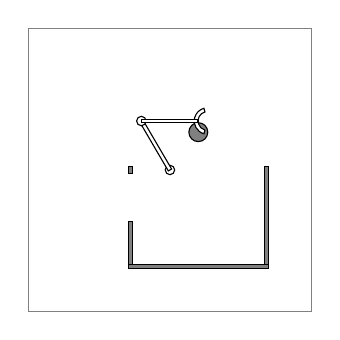
\begin{tikzpicture}
\begin{scope}[scale=1.2]
% bounding rect
\draw[color=black!50, thin] (-1.5,-1.5) rectangle (1.5,1.5);
\tikzstyle{dstyle}=[draw=black,fill=black!50]
\draw[dstyle] (0.300000,0.400000) circle (0.100000);
\draw[dstyle, shift={(0.300000,-1.020000)}, rotate=0.000000] (-0.740000,-0.020000) rectangle (0.740000,0.020000);
\draw[dstyle, shift={(1.020000,-0.480000)}, rotate=0.000000] (-0.020000,-0.520000) rectangle (0.020000,0.520000);
\draw[dstyle, shift={(-0.420000,-0.775000)}, rotate=0.000000] (-0.020000,-0.225000) rectangle (0.020000,0.225000);
\draw[dstyle, shift={(-0.420000,0.000000)}, rotate=0.000000] (-0.020000,-0.040000) rectangle (0.020000,0.040000);

\tikzstyle{dstyle}=[draw=black,fill=white]
\draw[dstyle] (0.000000,0.000000) circle (0.050000);
\draw[dstyle, shift={(-0.151454,0.258963)}, rotate=120.321137] (-0.300000,-0.020000) rectangle (0.300000,0.020000);
\draw[dstyle] (-0.302908,0.517926) circle (0.050000);
\draw[dstyle, shift={(0.397092,0.517926)}, rotate=180.000000](-74.484513:0.100000) arc (-74.484513:74.484513:0.100000) --(74.484513:0.140000) arc (74.484513:-74.484513:0.140000) -- cycle;
\draw[dstyle, shift={(-0.002908,0.517926)}, rotate=0.000000] (-0.300000,-0.020000) rectangle (0.300000,0.020000);

\end{scope}
\end{tikzpicture}
\caption{Invalid configuration}
\end{subfigure}%
\caption{Illustration of solution.}
\end{figure}

If we put some text in here, it shows up in the right place.

\begin{itemize}
\item comes from structure of multi-step problem
\item different cfrees
\item but they're very related!
\item inclusions, intersections
\end{itemize}

See Figure~\ref{fig:multi-set-example} for a simple motivating example.

\begin{figure}
\centering
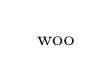
\begin{tikzpicture}

\node (a) at (0,0) {woo};

\end{tikzpicture}
\caption{An example of different $\mathcal{C}_{\mbox{\scriptsize free}}$s}
\label{fig:multi-set-example}
\end{figure}

\subsection{Multiple sub-queries}

\subsection{Shared C-space}

\subsection{Each in a different C-free}

\subsection{Relations between C-frees (inclusion, intersection)}

\section{Related Work}

The topic of reusing planning computation
between similar motion planning problems
has been extensively studied in different domains.

\subsection{Explicit Configuration Spaces}

Early planning methods constructed explicit obstacles
directly in the configuration space.
This allows reuse via precomputed bitmaps
for translating robots \cite{kavraki1995cspacefft}
or via workspace primitives \cite{newmanbranicky1991cspacetransforms}.
One form of reuse is to precompute these for primitives.
More recently,
Lien and Lu \cite{lien2009similarobstacles} describe a method to
build a PRM around obstacles in a database,
and then reposes them in a new world.
The approach is not easily applicable to articulated robots
with complex mappings from workspace to C-space.

\subsection{Changing Free $\mathcal{C}$-Subsets}

Other approaches attempt to prune and grow graphs
within dynamically changing collision-free subsets,
e.g. the Dynamic RRT \cite{ferguson2006drrt},
the Reconfigurable Random Forest (RRF)
\cite{li2002incrementalprmmanagement},
and the Lazy Reconfiguration Forest
\cite{gayle2007lazyreconfigforest}.
%We do the lazy thing as well (built into our planner).
%None of these reason about the structure of the configuration space.
However, these approaches do not reason explicitly about the
structure of the configuration space.

\subsection{Static vs Dynamic Components of
   $\mathcal{C}_{\mbox{\scriptsize free}}$}

Some approaches do take advantage of such structure
through a two-level dichotomy between
permanent and non-permanent parts of
$\mathcal{C}_{\mbox{\scriptsize free}}$.
Leven and Hutchinson \cite{leven2000changing}
and similar work \cite{kallman2004dynamicroadmaps}
handle changing environments by
precomputing a self-collision-free roadmap,
and then pruning it at query time
using a mapping from workspace cells to roadmap edges.
%This can also be viewed through the multi-space lens
%-- I think this is just an instantiation of a bunch of sets.
%They're very focused on the precomputation stuff.
%However, this approach this can't directly handle grasped objects.
Other methods \cite{jaillet2004dynamicprm}
exploit the dichotomy between static and dynamic parts of
the world online.

\subsection{Task and Motion Planning}

The structure in manipulation tasks that our approach leverages
is similar to the \emph{conditional reachability graph} which is
part of the recent \textsc{FFRob} heuristic task planning framework.
However, the framework is not incentivized to explore
areas of the configuration space that have already been explored.

\subsection{Fast Collision Checking}

Broad-phase collision checking.
See Section~\ref{subsec:broad-phase} for more on this.
I need cites!

\subsection{Sampling Strategies}

Also Kurniawati and Hsu's
\emph{Workspace-based Connectivity Oracle}
\cite{kurniawati2008workconnoracle}
which is a smart sampling strategy which considers workspace
geometry to inform PRM sampling.
Kurniawati has a bunch of other work on PRM fundamentals and sampling.
I think our approach is complementary to a PRM sampling strategy.
Or, you could do deterministic sampling
\cite{lavalle2002gridprms} \cite{geraerts2002prmcomparison}.

\subsection{Multi-Resolution Planning}

\noindent
\begin{itemize}
\item S. Kambhampati 1986
\item R. Steffens 2010
\item S. Zickler 2010
\item K. Gochev 2013
\end{itemize}

\subsection{Graph Search}

Many graph-search approaches are relevant to planning in similar
environments.
Algorithms such as
D* \cite{stentz1994dstar}
or LPA* \cite{koenig2004lpastar}
handle dynamically changing (or incrementally discovered) worlds.
Experience graphs \cite{phillips2012egraphs} are a method to apply
computation from previous graph-search planning queries
to the current problem.
The \textsc{BUGSY} algorithm \cite{ruml2007bugsy}
is most similar to our approach in the way that it explicitly
trades off between planning and execution (solution) cost.

\subsection{Other Related Work to Integrate}

Symbolic planning frameworks.

Newman and Branicky,
\emph{Real-Time Configuration Space Transforms for Obstacle Avoidance}
\cite{newmanbranicky1991cspacetransforms}
is a way to reuse stuff in related worlds.
From Sidd:
\begin{quote}
i know i've told you this before,
but it reminds me of how back in the day
people used to construct cobs
by stamping together cobs for primitives;
it's a form of reuse;
caching old cobs and transforming them for new problems

Here's a paper that talks about approximating C-obstacles.
They have a nice [obvious] theorem in 5.2. Set Containment Property.
\end{quote}

Also \cite{kavraki1995cspacefft}?

Also Kurniawati and Hsu's
\emph{Workspace-based Connectivity Oracle}
\cite{kurniawati2008workconnoracle}
which is a smart sampling strategy which considers workspace
geometry to inform PRM sampling.
Kurniawati has a bunch of other work on PRM fundamentals and sampling.

Jaillet and Simeon,
\emph{A PRM-based motion planner for dynamically changing environments}
\cite{jaillet2004dynamicprm}.
Explicit dichotomy between static and dynamic parts of the world.
Edges are checked when needed against moving obstacles;
their free-ness with respect to each is cached for the last tested position
for each obstacle.

Gayle, Klingler, and Xavier,
\emph{Lazy Reconfiguration Forest}
\cite{gayle2007lazyreconfigforest}.

Li and Shie,
\emph{An incremental learning approach to motion planning with
      roadmap management}
\cite{li2002incrementalprmmanagement}.
This is the Reconfigurable Random Forest (RRF).
They do ``roadmap management'' to handle changing environments,
and talk about doing some simple bounding-box stuff.

Lien and Lu,
\emph{Planning motion in environments with similar obstacles}
\cite{lien2009similarobstacles}.
This builds a PRM around obstacles in a database,
and then reposes them in a new world.

This is very similar to the \emph{conditional reachability graph}
presented by Garrett, Lozano-Perez, and Kaelbling
\cite{garrett2014ffrob}
as part of their task and motion symbolic planning mumbo-jumbo!

Also similar to the way changing environments are handled in PRMs
from Leven and Hutchinson \cite{leven2002changing}.

\section{Multi-Set Problem Formulation}
\label{sec:multi-set}

\begin{figure*}
\begin{widepage}
\centering

\begin{subfigure}[t]{.32\linewidth}
\centering
\includegraphics{build/figstar-a}
\caption{A two-part multi-set problem in $\mathcal{C}$,
  first between $x_1$ and $x_2$ through $X_{12}$,
  then between $x_2$ and $x_3$ through $X_{23}$.
  The two free sets $X_{12}$ and $X_{23}$ are distinct
  but related.}
\end{subfigure}%
\quad%
\begin{subfigure}[t]{.32\linewidth}
\centering
\includegraphics{build/figstar-b}
\caption{The free sets are related via other underlying
  subsets of $\mathcal{C}$, with $X_{12}=A \cap B$
  and $X_{23}=A \cap C$.
  A planner solving the first part (from $x_1$ to $x_2$)
  has found paths within $X_{12}$.}
\label{subfig:figstar-intersections}
\end{subfigure}%
\quad%
\begin{subfigure}[t]{.32\linewidth}
\centering
\includegraphics{build/figstar-c}
\caption{Due to the set relations,
  a planner solving the second part
  (from $x_2$ to $x_3$ in $X_{23}$)
  can reuse any segment known to be in $X_{12}$
  by checking only for its membership in $C$.}
\end{subfigure}

\vspace{0.1in}

\begin{subfigure}[t]{.32\linewidth}
\centering
\includegraphics{build/example-2d-a}
\includegraphics{build/example-2d-b}
\includegraphics{build/example-2d-c}
\caption{A forklift in a parking lot ($x_1$)
  must retrieve an object ($x_2$)
  and reverse park ($x_3$).
  This two-part problem
  requires plans in distinct collision-free
  $\mathcal{C}$-subsets
  $X_{12}$ and $X_{23}$.}
\label{subfig:figstar-manip-probdef}
\end{subfigure}%
\quad%
\begin{subfigure}[t]{.32\linewidth}
\centering
\includegraphics{build/example-2d-d}
\includegraphics{build/example-2d-e}
\includegraphics{build/example-2d-f}
\caption{Sets $X_{12}$ and $X_{23}$ are subsets of
  the configuration space of the robot $\mathcal{C}=\mbox{SE}(2)$,
  and can be represented as intersections
  of underlying subsets $A$, $B$, and $C$
  as in Fig.~\ref{subfig:figstar-intersections}.}
\label{subfig:figstar-manip-spaces}
\end{subfigure}%
\quad%
\begin{subfigure}[t]{.32\linewidth}
\centering
\includegraphics{build/example-2d-g}
\includegraphics{build/example-2d-h}
\includegraphics{build/example-2d-i}
\caption{After planning a path from $x_1$ to $x_2$ (top),
  a planner can reuse a configuration in $X_{12}$ (middle)
  by checking only for its membership in subset $C$,
  resulting in plan reuse (bottom).}
\end{subfigure}

\caption{An illustration of a multi-set planning
  problem in a common configuration space $\mathcal{C}$.
  The problem definition generalizes to an artibrary number of
  configuration space subsets and set relations between them.
  When two queries in different subests are solved sequentially,
  a multi-set planner can reuse path segments less expensively.
  See Section~\ref{sec:in-manipulation} for examples in
  manipulation.}
\label{fig:multi-set}
\end{widepage}
\end{figure*}

Here we define the multi-set planning problem,
a generalization of both the movers' problem
and the multi-query planning problem
\cite{kavrakietal1996prm}.
The reader is referred to
Fig.~\ref{fig:multi-set}
for a general example,
as well as a simple instantiation in a 2D manipulation task.
%which is discussed in more detail in
%Section~\ref{subsec:multi-prm-example}.
The multi-set problem formulation
explicitly captures both planning and
solution (execution) cost.

\subsection{Formal Multi-Set Problem Definition}
\label{subsec:problem-definition}

The multi-set planning problem is multi-query in
a fixed configuration space $\mathcal{C}$.
However, unlike related problems in which all
queries demand solution paths contained within a single common subset of
$\mathcal{C}$
(usually the set of collision-free configurations, denoted
$\mathcal{C}_{\mbox{\scriptsize free}}$),
the multi-set problem allows for the specification of
\emph{multiple} such $\mathcal{C}$-subsets
$\mathcal{S} = \{ A, B, \dots \}$.
Like $\mathcal{C}_{\mbox{\scriptsize free}}$,
each member of $\mathcal{S}$
is a subset of the common configuration space
(that is,
$X \subseteq \mathcal{C} \;\forall\; X \in \mathcal{S}$).
For example, in Fig.~\ref{subfig:figstar-manip-spaces},
$\mathcal{C}$-subset $B$
consists of configurations
free of collision between the robot and
the initial object pose.

\begin{figure}
\centering
\begin{subfigure}[t]{0.45\linewidth}
\centering
\includegraphics{build/query-to-subset-a}
\caption{Multi-query planning}
\end{subfigure}%
\quad\quad%
\begin{subfigure}[t]{0.45\linewidth}
\centering
\includegraphics{build/query-to-subset-b}
\caption{Multi-set planning}
\end{subfigure}
\caption{While queries in multi-query planning reference
  the same subset of $\mathcal{C}$,
  each multi-set query references one of a number of such sets.}
\label{fig:query-to-subset}
\end{figure}

The problem supports an arbitrary number of queries $\mathcal{Q}$.
Each query $q$ references a \emph{single}
$\mathcal{C}$-subset $X_q \in \mathcal{S}$
(see Fig~\ref{fig:query-to-subset}):
\begin{equation}
  q : ( x_{start},\; x_{goal},\; X_q ) .
  \label{eqn:q}
\end{equation}
A continuous feasible solution path $x(t)$ must then satisfy
\begin{equation}
  \begin{array}{c}
  x(t) \in X_q \;\forall\; t \in [0,1] \\
  x(0) = x_{start},\; x(1) = x_{goal} . \\
  \end{array}
  \label{eqn:solution}
\end{equation}
Eqns. (\ref{eqn:q}), (\ref{eqn:solution})
specify single configurations
$x_{start}$ and $x_{goal}$,
but the formulation is trivially extended to start/goal sets.

While simple problems may admit explicit representations of
subsets of $\mathcal{C}$,
recent approaches to complex problems
(e.g. sampling-based planners)
instead reason implicitly via test function(s)
\cite{lavalle2006planningbook}.
To capture this,
we endow each $\mathcal{C}$-subset $X \in \mathcal{S}$ with an
\emph{indicator function} $\mathbf{1}_X(x)$:
\begin{equation}
  \mathbf{1}_X(x) =
    \left\{ \begin{array}{ll}
      \mbox{True} & \mbox{if } x \in X \\
      \mbox{False} & \mbox{otherwise}.
    \end{array} \right.
  \label{eqn:indicator-function}
\end{equation}
Equivalently, the set itself can be defined w.r.t. its indicator:
\begin{equation}
  X = \{ x \in \mathcal{C} \;|\; \mathbf{1}_X(x) = \mbox{True} \} .
\end{equation}
Excusing the abuse of notation,
we define an analogous indicator functional $\mathbf{1}_X[\cdot]$
which operates on path segments $x(t)$.
We use parentheses for functions and brackets for functionals.
\begin{equation}
  \mathbf{1}_X[x(t)] =
    \left\{ \begin{array}{ll}
      \mbox{True} & \mbox{if } x(t) \in X \;\forall\; t \in [0,1] \\
      \mbox{False} & \mbox{otherwise}.
    \end{array} \right.
  \label{eqn:indicator-functional}
\end{equation}
Common examples of such indicators
(\ref{eqn:indicator-function}) or (\ref{eqn:indicator-functional})
include validity checkers for
geometric (workspace) collision,
stability, and visibility constraints.
Note that for complex problems,
evaluation of these indicators 
tends to dominate planning cost.

\begin{figure}
\centering
\begin{subfigure}[t]{0.45\linewidth}
\centering
\includegraphics{build/relations-inclusion} \\
$A \subseteq B$ \\
$\mathbf{1}_A \Rightarrow \mathbf{1}_B$
\caption{Containment relation}
\end{subfigure}%
\quad\quad%
\begin{subfigure}[t]{0.45\linewidth}
\centering
\includegraphics{build/relations-intersection} \\
$A = B \cap C$ \\
$\mathbf{1}_B \wedge \mathbf{1}_C \Rightarrow \mathbf{1}_A$
\caption{Intersection relation}
\end{subfigure}
\caption{Types of relations used in the paper.
  Each relation can be expressed directly as set relations
  or equivalently as logical statements
  on the corresponding indicator functions
  $\mathbf{1}_X(\cdot)$.}
\label{fig:relations}
\end{figure}

Finally, the multi-set problem incudes a list of set relations
$\mathcal{R}$
between the $\mathcal{C}$-subsets in $\mathcal{S}$.
These can be expressed directly using set theoretic relations,
or equivalently as logical statements
on the corresponding indicator functions.
The two types of relations we use in this paper
(containment and intersection)
are described in Fig.~\ref{fig:relations}.
Fig.~\ref{fig:multi-set} gives an example of intersection relations;
an example of containment is a padded (conservative)
robot model (see Section~\ref{subsec:broad-phase}).

Together, these four elements
(a configuration space $\mathcal{C}$,
subsets $\mathcal{S}$ each with endowed indicators,
a set of queries $\mathcal{Q}$,
and a list of subset relations $\mathcal{R}$)
comprise a multi-set planning problem.

\subsection{Cost Model}
\label{subsec:cost-model}

While the indicators
(\ref{eqn:indicator-function}) and (\ref{eqn:indicator-functional})
are binary,
we are often interested not only in solution feasibility,
but also minimizing a measure of \emph{execution cost}
on the solution path.
Furthermore,
\emph{planning cost} is often also an important consideration.
Here,
we define a cost model $\mathcal{M}$
for multi-set problems
which allows these costs to be captured.

\subsubsection{Execution Cost}
We capture the expected execution cost of a candidate path
$x(t)$ in the space of $\mathcal{C}$-space paths $H$
via a simple functional
\begin{equation}
  f_e : H \rightarrow \mathbb{R}_0^+ .
\end{equation}
We assume that $f_e[x(t)]$ is known and inexpensive to compute.
Common metrics include
execution time (s) or energy (J).

\subsubsection{Planning Cost}
Since indicator evaluation tends to dominate planning costs
in sampling-based planners,
we choose to explicitly penalize such evaluations.
In particular,
each call to indicator functional $\mathbf{1}_X[\cdot]$
incurs a cost given by $f_X[\cdot]$:
\begin{equation}
  f_X : H \rightarrow \mathbb{R}_0^+ .
\end{equation}
We assume that $f_X[\cdot]$ itself is inexpensive to compute.
Common estimates include expected collision checking time (s)
or computational energy required (J).
Often, $f_X[x(t)]$ is proportional to both
the length of the path $x(t)$
and a fixed estimate of the complexity of $\mathcal{C}$-subset $X$.

Together, the execution cost functional $f_e$
and the planning cost functionals $f_X \;\forall\; X \in \mathcal{S}$
comprise the multi-set cost model $\mathcal{M}$.
Note that representing all functionals in common units
(e.g. seconds or Joules) allows a planners
(e.g. the Multi-Set PRM in Section~\ref{chap:multi-set-prm})
to effectively trade off between planning and execution cost.

\subsection{Example Problem}
\label{subsec:multi-prm-example}

Consider the diagram from Fig.~\ref{fig:multi-set}.
$\mathcal{S}$ consists of five $\mathcal{C}$-subsets labeled
$A$, $B$, $C$, $X_{12}$, and $X_{23}$,
and we have two queries,
$q_{12}: (x_1, x_2, X_{12})$
and
$q_{23}: (x_2, x_3, X_{23})$.
$\mathcal{R}$ consists of the two relations
$X_{12} = A \cap B$ and $X_{23} = A \cap C$.
Suppose a cost model $\mathcal{M}$
wherein evaluating the indicator
$\mathbf{1}_A$ incurs cost 4,
evaluating $\mathbf{1}_B$ and $\mathbf{1}_C$ incurs cost 2,
and evaluating $\mathbf{1}_{X_{12}}$ and $\mathbf{1}_{X_{23}}$
incurs cost 6.
In the manipulation example in
Fig.~\ref{subfig:figstar-manip-probdef},
this would be the case if each
pairwise outlined shape collision check incurs unit cost.

Suppose a graph structure within ${X_{12}}$ has been grown to solve
the first query $q_{12}$.
During the subsequent solve of query $q_{23}$,
an existing path segment known to be in ${X_{12}}$ can be shown to
also be contained within ${X_{23}}$ by only evaluating $\mathbf{1}_C$.
In the manipulation example,
reusing an a configuration from the previous search
would require only a check of cost 2,
instead of cost 6 for a new configuration.
Thus, we might hope that a planner may be biased towards reusing
said edges in this case.

For a list of example multi-set problems which arise in manipulation
tasks,
see Section~\ref{sec:in-manipulation}.

\section{Multi-Set Problems in Manipulation Tasks}
\label{sec:in-manipulation}

Instances of multi-set problems are especially prevalent when
planning for manipulation tasks with articulated robots.
This section details several such instances.
While these instances are discussed separately here,
they are often present simultaneously.
See Section~\ref{subsec:herb-experiment}
for experimental results for a problem
which includes several of the multi-set problem instances
described below.

We also provide an implementation for the
OpenRAVE\cite{diankov2010openrave}
virtual kinematic planning environment
which automatically discovers $\mathcal{C}$-subsets
in manipulation tasks.

\subsection{Dynamic Environments}
\label{subsec:dynamic-environments}

\begin{figure}
\centering

\begin{subfigure}[b]{\linewidth}
\centering
\begin{tikzpicture}
\tikzset{>=latex} % arrow heads
\node[anchor=south west,inner sep=0] at (0,0)
  {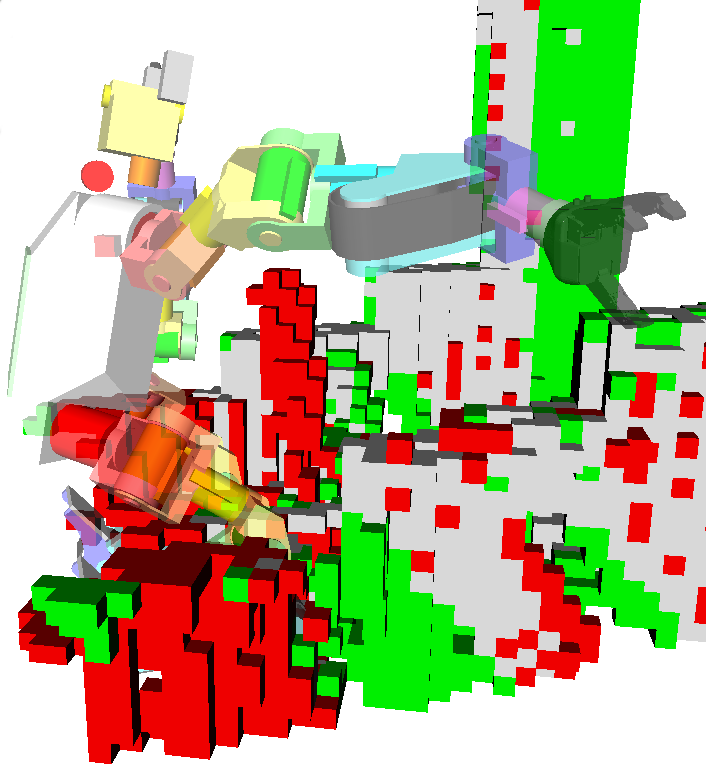
\includegraphics[width=0.56\columnwidth]{figs/chimp-voxels-delta.png}};

\node[draw,inner sep=3pt,fill=white,fill opacity=0.9,align=center]
  (debrislab) at (-0.7,3.5) {Debris object\\removed};
\node[circle,inner sep=2,draw,fill=white] (debris) at (2.0,2.9) {};
\draw[draw=black, double=white, double distance=1pt, line width=1pt]
  (debrislab.east) -- (debris);
  
\node[draw,inner sep=3pt,fill=white,fill opacity=0.9,align=center]
  (debrislab) at (5.8,5.2) {Additional\\voxels seen};
\node[circle,inner sep=2,draw,fill=white] (debris) at (4.2,5.0) {};
\draw[draw=black, double=white, double distance=1pt, line width=1pt]
  (debrislab.west) -- (debris);
  
\end{tikzpicture}
\caption{A disaster response robot maintains a
  dynamic unstructured environment model
  using coarse voxels
  (scene data from a debris-clearing task at a
  recent disaster response competition).
  Since the last planning query,
  voxels have been added (green) and removed (red).}
\label{fig:chimp-voxels-delta}
\end{subfigure}

\vspace{0.1in}

\begin{subfigure}[b]{\linewidth}
\centering
\includegraphics{build/retroactive-a}
\includegraphics{build/retroactive-b}
\caption{
  $\mathcal{C}$-subsets and relations
  can be added retroactively.
  Here, the graph for an initial query is checked w.r.t $X_1$.
  After environment changes,
  $X_1$ is redefined in terms of the $\mathcal{C}$-subsets
  derived from the set of common, added, and removed elements,
  allowing for reuse on a query in $X_2$.
  Here,
  the planner need only check existing path segments
  against added voxels in order to reuse them for the current query.}
\label{fig:retroactive}
\end{subfigure}

\caption{
  Structured or unstructured dynamic environments
  can be represented as a multi-set problem
  (see Section~\ref{subsec:dynamic-environments}).}
\label{fig:dynamic-environments}
\end{figure}

The sensors on most articulated robots allow them to maintain
dynamic environment models to track changing collision geometry
(see Fig.~\ref{fig:chimp-voxels-delta}).
These models might be
structured (e.g. recognizing objects with known models)
or unstructured (e.g. occupancy models).
In both cases,
even in a changing world,
there are often areas that are fixed between planning queries.

Prior work (e.g. \cite{jaillet2004dynamicprm})
leverages this by imposing a dichotomy between
\emph{fixed} and \emph{moving} components of $\mathcal{C}$.
Our formulation extends this to an arbitrary number of such labels,
including ones defined retroactively (i.e. during planning;
see Fig.~\ref{fig:retroactive}).
By explicitly labeling such areas in workspace
(and leveraging the \emph{set containment} property
\cite{newmanbranicky1991cspacetransforms}),
we can represent this structure as a multi-set planning problem.

Special case of this is if objects are disappearing.

Relation to occupancy grid representations of workspace
(for deltas, conservative approxs, etc).

\subsection{Grasped Objects}
\label{subsec:grasped-objects}

One instance specific to manipulation problems is the handling of
grasped objects.
For example, 
consider a manipulator which grasps a geometric object.
This affects the set of collision-free configurations
across a large section of $\mathcal{C}$
relative to the old set of valid configurations $X_{old}$.
However,
the resulting $\mathcal{C}$-subset $X_{new}$
can be represented simply as
$X_{new} = X_{old} \cap G$,
with $G$ the set of robot configurations in which
the \emph{grasped object} (only)
is deemed free of collision with the robot and environment.
This structure is discussed in the context of the
\emph{conditional reachability graph},
part of the \textsc{FFRob} heuristic framework
\cite{garrett2014ffrob}.

For example,
consider the manipulation problem in
Figure~\ref{fig:testherb-problem}.
The robot must find a path which moves its arm to grasp the cup.
After the cup is grasped,
the robot can reuse any edge in the existing roadmap
but simply checking the grasped cup
against the remainder of the environment.
This structure,
together with the approach to dynamic environments,
are included together in the experimental results
(Section~\ref{subsec:herb-experiment}).

\begin{figure}
\centering
\includegraphics{build/self-collision}
\caption{A roadmap is pre-computed in $R$,
  the subset of $\mathcal{C}$ consisting of configurations free
  of robot self-collision.
  Online, the planner must find a path that's also within $E$,
  the subset free of environment collision.
  When solving this query in $X = R \cap E$,
  the Multi-Set PRM automatically prefers potential paths with
  pre-computed edges (e.g. shown in grey)
  due to lower planning costs over alternatives with lower
  execution costs.}
\label{fig:self-collision-example}
\end{figure}

\subsection{Cached Self-Collision-Checked Roadmaps}
\label{subsec:cached-self-valid}

Self-collision checking is a potentially expensive component to
articulated motion planning;
in contrast to environment checking,
it is fundamentally quadratic in the number of moving links.
Further, pairs of links to be checked
tend to be relatively close to each other,
reducing the effeciveness of broad-phase approaches.

Leven and Hutchinson \cite{leven2000changing}
introduced the concept of a pre-cached roadmap consisting of
configurations and paths already known to be valid w.r.t.
self-collision.
As a type of invariant in $\mathcal{C}$,
this can be seen as a particular instance of multi-set planning.
See Fig.~\ref{fig:self-collision-example}.

\begin{figure}
\centering

\begin{subfigure}[t]{\linewidth}
\centering
\includegraphics{build/broadphase-single}
\caption{A single-set planner testing simply for membership in
  $\mathcal{C}_{\mbox{\scriptsize free}}$
  treats a collision validity checker as a
  ``black box.''
  Internally,
  modern checkers first employ an inexpensive broad-phase check
  using a low-dimensional conservative representation
  to quickly identify non-colliding bodies before
  resorting to an expensive narrow-phase check.}
\end{subfigure}

\vspace{0.2in}

\begin{subfigure}[t]{\linewidth}
\centering
\includegraphics{build/broadphase-multi}
\caption{A multi-set planner can explicitly reason about the
  conservative nature of the broad-phase check.
  This allows it to defer some narrow phase checks
  (often indefinitely)
  and instead prefer paths that require fewer expensive checks.}
\end{subfigure}

\caption{Collision validity checking is a commonly used
  indicator function.
  The multi-set formulation allows an intelligent planner to
  reach inside the checker's ``black box'' and reduce the number
  of costly narrow-phase checks.
  Resulting paths tend to be cheaper to compute and
  stay further from obstacles.}
\label{fig:broad-phase}
\end{figure}

\subsection{Integration with Broad-Phase Collision Checking}
\label{subsec:broad-phase}

\begin{figure}
\centering

\begin{subfigure}[t]{0.45\linewidth}
\centering
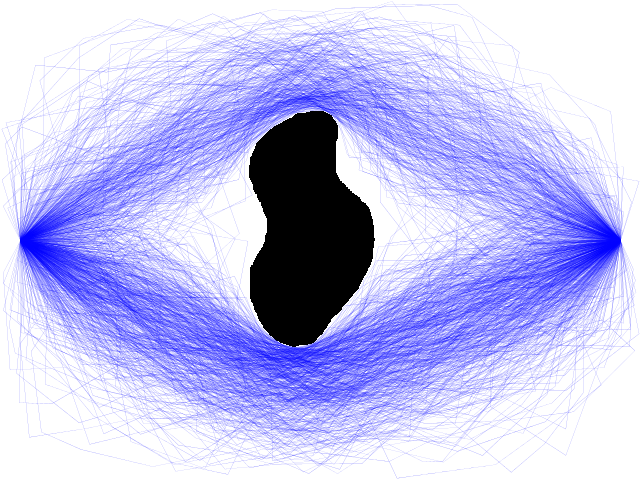
\includegraphics[width=\columnwidth]{figs/paths-lambda0-norel.png}
\caption{
  $\lambda=0$, no broad phase.\\
  Median planning cost: 6650}
\end{subfigure}
\begin{subfigure}[t]{0.45\linewidth}
\centering
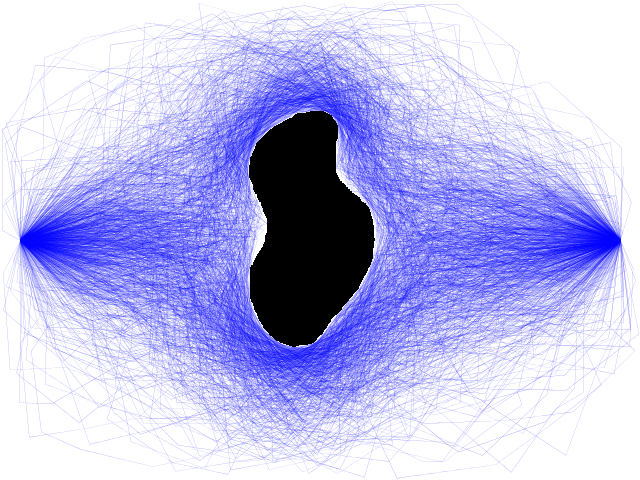
\includegraphics[width=\columnwidth]{figs/paths-lambda1-norel.png}
\caption{
  $\lambda=1$, no broad phase.\\
  Median planning cost: 4530}
\end{subfigure}

\begin{subfigure}[t]{0.45\linewidth}
\centering
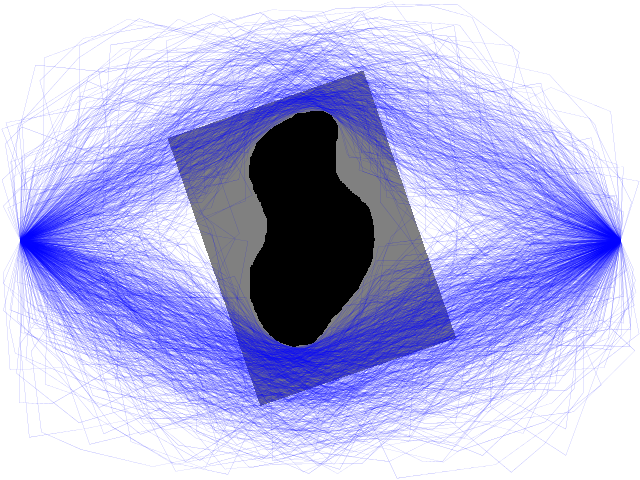
\includegraphics[width=\columnwidth]{figs/paths-lambda0-wrel.png}
\caption{
  $\lambda=0$, with broad phase.\\
  Median planning cost: 2122}
\end{subfigure}
\begin{subfigure}[t]{0.45\linewidth}
\centering
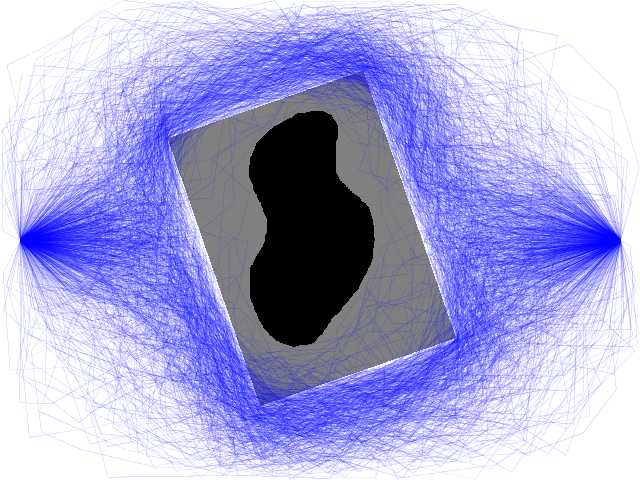
\includegraphics[width=\columnwidth]{figs/paths-lambda1-wrel.png}
\caption{
  $\lambda=1$, with broad phase.\\
  Median planning cost: 737}
\end{subfigure}

\caption{A simple 2D example of the Multi-Set PRM using
  a broad-phase check.
  Checking for collision with the grey box is 10x less expensive
  than with the actual black obstacle.
  \cdnote{I need to talk about this in the text.}}
\label{fig:broad-phase-2d}
\end{figure}

The multi-set formulation also enables motion planners to
reason directly about different robot or environment models.
For example, consider two geometric robot models,
one with high quality (e.g. from a CAD program),
and one hand-tuned ``padded'' model consisting of 
a small number of simple conservative bounding volumes.
The $\mathcal{C}$-subsets derived from these models,
are related by $R_{padded} \subseteq R_{CAD}$.
Collision checkers currently use a similar approach internally
to speed up collision checks (see Fig.~\ref{fig:broad-phase}.
and Fig~\ref{fig:broad-phase-2d}).

\subsection{Conservative Bounding Volumes for Different Grasps}

\subsection{Conservative Bounding Volumes for Hypothesized Objects}

There's a sweet ICRA paper here.

\subsection{Dual Arm Stuff}

I think this is related.

Check right arm against gian left side box, etc.

\subsection{Dimensionality Reduction}

The Handey \cite{lozanoperez1987handey} robot
assumed a box that contained the wrist links at a range of DOF values.

\section{Other Stuff}

Potential research question: learn cost model over time.
